\section{Experiment 5: Mathematical analysis and simulation of a 1D network}
\label{section:1D}

\subsection{Introduction}

The purpose of this experiment was to mathematically analyse a simpler network, thus providing a definitive way to verify the performance of the simulation. The network was scaled down to be one-dimensional with 18 input neurons, four prior neurons and four output neurons, making it easier to analyse. The conditional probabilities of the input and output neurons of the network  were calculated by hand and then used to determine the theoretical posterior probability of the network. These probabilities were then used to calculate the weights for the simulation of the network. The distribution of the output spikes was then used to calculate the posterior probability of the simulation. The posterior probabilities of both the mathematical analysis and the simulation are compared, and by varying three parameters of the simulation it is tuned to approximate the analytical solution as closely as possible.

\subsection{Methods}

\paragraph{Network structure}
The architecture of this network remained the same as in previous experiments (with adaptive inhibition and a noise level of 10\%), only the amount of neurons was changed. The input image consists of nine pixels in a horizontal line. Within those nine pixels four output classes can be represented. Each output class consists of three pixels next to each other. This results in each output class overlapping its neighbour classes by one pixel. Thus the centres of the output classes are at position 1, 3, 5 and 7.    As there have to be 2 input neurons for each pixel, one neuron being active if the pixel is white and one if the pixel is black, the network has 18 input neurons. Furthermore four prior neurons were implemented, of which only one is being active for one of the output classes at a time. Lastly the network has four output neurons.

\paragraph{Mathematical Analysis}
The posterior probability of the network was calculated by using
\begin{equation}
\label{eqn:pYvorausgesetztXUndZ}
P(Y = i|X = x, Z = j) = \frac{P(X=x|Y=i)P(Y = i|Z = j)}{\Sigma_{k}P(X=x,Y=k)P(Y=k|Z=j)}.
\end{equation}
$P(X=x|Y=i)$ and $P(Y=i|Z=j)$ were derived by hand corresponding to the paradigm of the experiment. The calculation of $P(X=x|Y=i)$ was split into two parts. First the contribution of the active input neurons was calculated by determining the matrix $P^{X|Y}$. This matrix is of size 4 x 9 and contains the conditional probabilities of each input neuron $y_i$ being active, given that an output neuron $x_l$ is active. These probabilities were calculated by determining which input neurons are active depending on the output class and which input neurons are inactive, as dictated by the network structure.  Furthermore the noise that was applied to the input neurons had to be taken into account. For input neurons belonging to the output class the conditional probability was determined as 1 and lowered by the noise level, while for the input neurons outside of the 3-wide pixel block belonging to the output class it was determined as 0 and raised by the noise level. According to this algorithm $P^{X|Y}$ is given by
\begin{equation}
\label{eqn:PXvorausgesetztYIf}
P_{i,l}^{X|Y} = \begin{dcases*} 1 - $noise level$ & if $x_l$ is in the active area of $y_i$, \\
0 + $noise level$ & \text{if $x_l$ is not in the active area of $ y_i $ } \end{dcases*}.\end{equation}
  After calculating all entries of $P^{X|Y}$ its rows were multiplied with the input image vector
\begin{equation}
\label{eqn:p1XvorausgesetztYMalX}
P_1(X = x|Y = i) = P^{X|Y}_{i,*} \cdot x
\end{equation}
resulting in a conditional probability for each output class depending on the input vector. The input vector was given with entries of 1 for active pixels and with entries of 0 for inactive pixels.
Next to include the contribution of the input neurons that are spiking when a pixel is inactive the conditional probability of the input neurons that are active for the entries where $x_i = 0$ had to be calculated. To achieve this complementary conditional probability at first $P^{X|Y}$ was subtracted from one. To include the correct conditional probabilities for the complementary case the input image vector x was then also subtracted from one. $1 - P^{X|Y}$ and $1 - x$ were multiplied to yield
\begin{equation}
\label{eqn:p2minusXvorausgesetztYMalX}
P_2(X = x|Y = i) = (1 - P^{X|Y}_{i,*}) \cdot (1 - x).
\end{equation}
The results of both calculations were then multiplied element-wise to yield
\begin{equation}
\label{eqn:pXvorausgesetztY}
P(X = x|Y = i) = P_1(X = x|Y = i) \odot P_2(X = x|Y = i).
\end{equation}
$P(Y=i|Z=j)$ was determined by first calculating the matrix $P^{Y|Z}$. It has a dimension of 4 x 4 and contains the conditional probabilities for the output neuron $y_i$, given the prior neuron $z_j$ being active. For each output class there exists one corresponding prior neuron. As there can never be more than one active prior neuron at a time $P^{Y|Z}$ is given by
\begin{equation}
\label{eqn:PYvorausgesetztZIf}
P_{j,i}^{Y|Z} = \begin{dcases*} 1 - $noise level$ & if $i = j$, \\
0 +  \frac{1}{3}  $noise level$ & \text{if $i \neq j$. } \end{dcases*}\end{equation} 
$P(Y=i|Z=j)$ was then obtained by
\begin{equation}
\label{eqn:pYvorausgesetztZ}
P(Y=i|Z=j) = P^{Y|Z} \cdot z
\end{equation}
where z is given by a 4 x 1 one-hot encoded vector of the prior.

\paragraph{Simulation}
The input weights for the simulation were calculated as two separate sets. First weights $w^{i1}$ for the input neurons that are active for active input pixels were determined by 
\begin{equation}
\label{eqn:1DWeights}
w^{i1} = \ln(P^{X|Y}).
\end{equation}
Second complementary input weights $w^{i2}$ were calculated for  input neurons representing non active input pixels with
\begin{equation}
\label{eqn:1DWeightsComplementary}
w^{i2} = \ln(1 - P^{X|Y}).
\end{equation} 
The prior weights $w^p$ were derived by 
\begin{equation}
\label{eqn:1DWeightsPrior}
w^p = \ln(P^{Y|Z}).
\end{equation}
The network was simulated for six different input images for each parameter set. After the image presentation period of each input image the amount of the output spikes of different classes were counted and their proportions were calculated to yield the "simulation output probabilities" in later plots. The Kullback-Leibler divergence was chosen to compare the divergence of the analytic and the simulated results of the network. This metric indicates how much two probability distributions diverge from each other. The goal of the parameter search of the simulation was to minimize the Kullback-Leibler divergence. Upon completion of the simulation of an output image the Kullback-Leibler divergence was calculated for that image
\begin{equation}
\begin{split}
\label{eqn:KLDivergence}
D_{KL}(P_{analysis}(Y = i|X, Z)||P_{simulation}(Y = i|X, Z)) = \\ \sum_{i=1}^K P_{analysis}(Y = i|X, Z) \cdot \ln( \frac{P_{analysis}(Y = i|X, Z)}{P_{simulation}(Y = i|X, Z)})
\end{split}
\end{equation}
where K is the number of output neurons and $P_{analysis}(Y = i|X, Z)$ and $P_{simulation}(Y = i|X, Z)$ are the "analysis output probabilities" and "simulation output probabilities". The six resulting Kullback-Leibler divergences for each parameter set were then averaged to create a single metric by which the performance of the different parameter sets was compared. The three parameters input firing rate $f_{input}$, prior firing rate $f_{prior}$ and the membrane constant $\tau_{decay}$ were varied to inspect their influence on the result, as well as to approximate the analytical solution as closely as possible. Each input image is presented to the network for 20 seconds to reduce the variance between runs. Furthermore each simulation was repeated 20 times with the same parameter set to obtain the mean and standard deviation of the simulation output probabilities and of the Kullback-Leibler divergence.

\subsection{Results}

\paragraph{Analytic Results}

First the matrix $P^{X|Y}$ was analytically calculated by using Equation \ref{eqn:PXvorausgesetztYIf} 
\begin{equation}
\label{eqn:pXvorausgesetztYResult}
P^{X|Y} = \begin{bmatrix}
0.9 & 0.9 & 0.9 & 0.1 & 0.1 & 0.1 & 0.1 & 0.1 & 0.1\\
0.1 & 0.1 & 0.9 & 0.9 & 0.9 & 0.1 & 0.1 & 0.1 & 0.1\\
0.1 & 0.1 & 0.1 & 0.1 & 0.9 & 0.9 & 0.9 & 0.1 & 0.1\\
0.1 & 0.1 & 0.1 & 0.1 & 0.1 & 0.1 & 0.9 & 0.9 & 0.9\\
\end{bmatrix}.
\end{equation}
Next the matrix $P^{Y|Z}$ was analytically calculated by using Equation \ref{eqn:PYvorausgesetztZIf} 
\begin{equation}
\label{eqn:pYvorausgesetztZResult}
P^{Y|Z} = \begin{bmatrix}
0.9 & 0.0333 & 0.0333 & 0.0333\\
0.0333 & 0.9 & 0.0333 & 0.0333\\
0.0333 & 0.0333 & 0.9 & 0.0333\\
0.0333 & 0.0333 & 0.0333 & 0.9\\
\end{bmatrix}.
\end{equation} 
For each input image these two matrices were then  multiplied with the input vector and prior vector as described Equations \ref{eqn:p1XvorausgesetztYMalX}, \ref{eqn:p2minusXvorausgesetztYMalX},  \ref{eqn:pXvorausgesetztY} and \ref{eqn:pYvorausgesetztZ} to yield $P(X = x|Y = i)$ and $P(Y=i|Z=j)$. Using  \ref{eqn:pYvorausgesetztXUndZ} then 
yielded $P(Y = i|X = x, Z = j)$ also called "Analysis output probabilities" in later plots.

\paragraph{Simulation results without prior}
To simplify the parameter fitting process the network was at first simulated with inactive prior neurons. Only after determining the best values for $f_{input}$ and $\tau_{decay}$ were the prior neurons reactivated and $f_{prior}$ was fitted. The values 0.015 seconds and 0.004 seconds for $\tau_{decay}$ were used for the simulation and compared. For each of these values an optimal value for $f_{input}$ was found by simulating different values and looking for the value that yields the smallest Kullback-Leibler divergence.

\subparagraph{$\tau_{decay} = 0.015 seconds$, $f_{prior} = 0 Hz$}
Values for $f_{input}$ between 10 and 110 Hz in steps of 10 Hz were simulated. After identifying the input firing rate with the smallest Kullback-Leibler divergence the network was simulated again for $f_{input}$ values $\pm$ 10 Hz in steps of 2 Hz of the best value. The result of this search can be seen in Figure \ref{fig:1D_KLD_fPrior0_tau15}. This process yielded the best input firing rate of 42 Hz. The results of this parameter combination can be seen in Figure \ref{fig:1D_42_0_15}. In this figure six different input images can be seen marked with the letter "A". The active pixels are shown in black.  The posterior probability of the mathematical analysis can be seen next to the letter "B". And finally the proportion of output spikes of the different output neurons can be seen next to the letter "C". Each probability of "C" has a standard deviation next to it, which was calculated over 20 runs of the network. At the bottom the value of the Kullback-Leibler divergence is given, with its standard deviation next to it.

\begin{figure}
  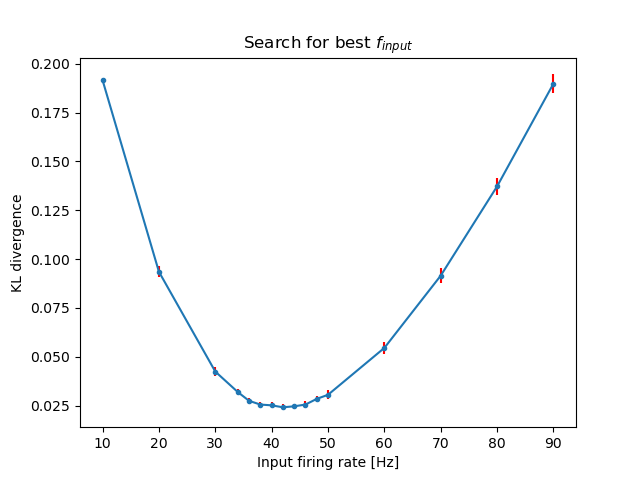
\includegraphics[width=\linewidth]{figures/1D/KLDvsfInput_fPrior0tau15.png}
  \caption{\textbf{KL divergence for different $f_{input} values$} $f_{prior} = 0 Hz, \tau_{decay} = 15 ms$}
  \label{fig:1D_KLD_fPrior0_tau15}
\end{figure}

\begin{figure}
  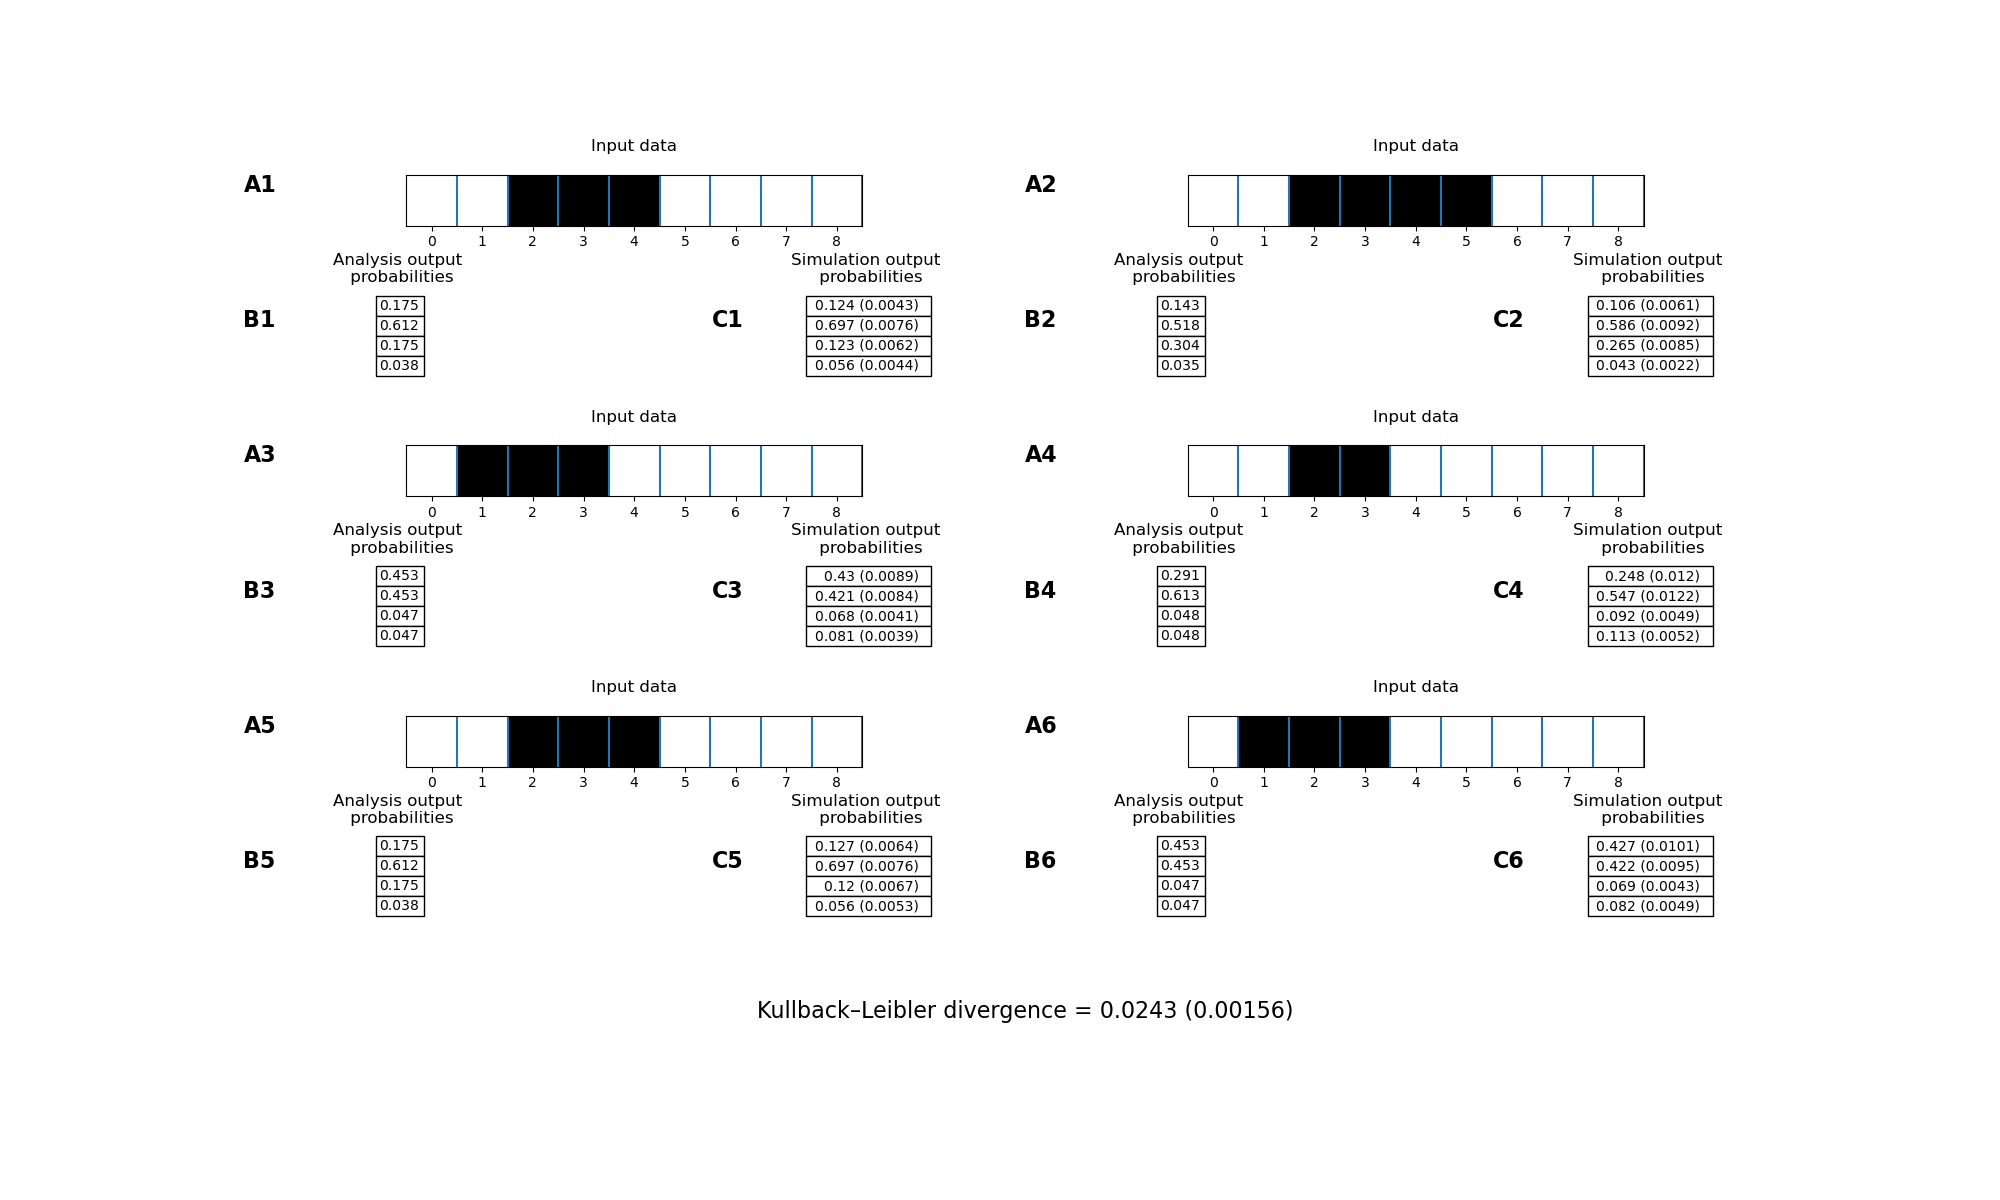
\includegraphics[width=\linewidth]{figures/1D/1D_42_0_15.png}
  \caption{\textbf{Analysis and simulation result. Parameters: } $f_{input} = 42 Hz, f_{prior} = 0 Hz, \tau_{decay} = 15 ms$ \textbf{A} Input images with 9 x 1 pixels. \textbf{B} Analytically calculated posterior probabilities. \textbf{C} Proportions of the spikes of the output neurons during the simulation and their standard deviations in brackets.}
  \label{fig:1D_42_0_15}
\end{figure}

When $f_{input}$ was 70 Hz the results of the analysis and the simulation differed more as can be seen in Figure \ref{fig:1D_70_0_15}.

\begin{figure}
  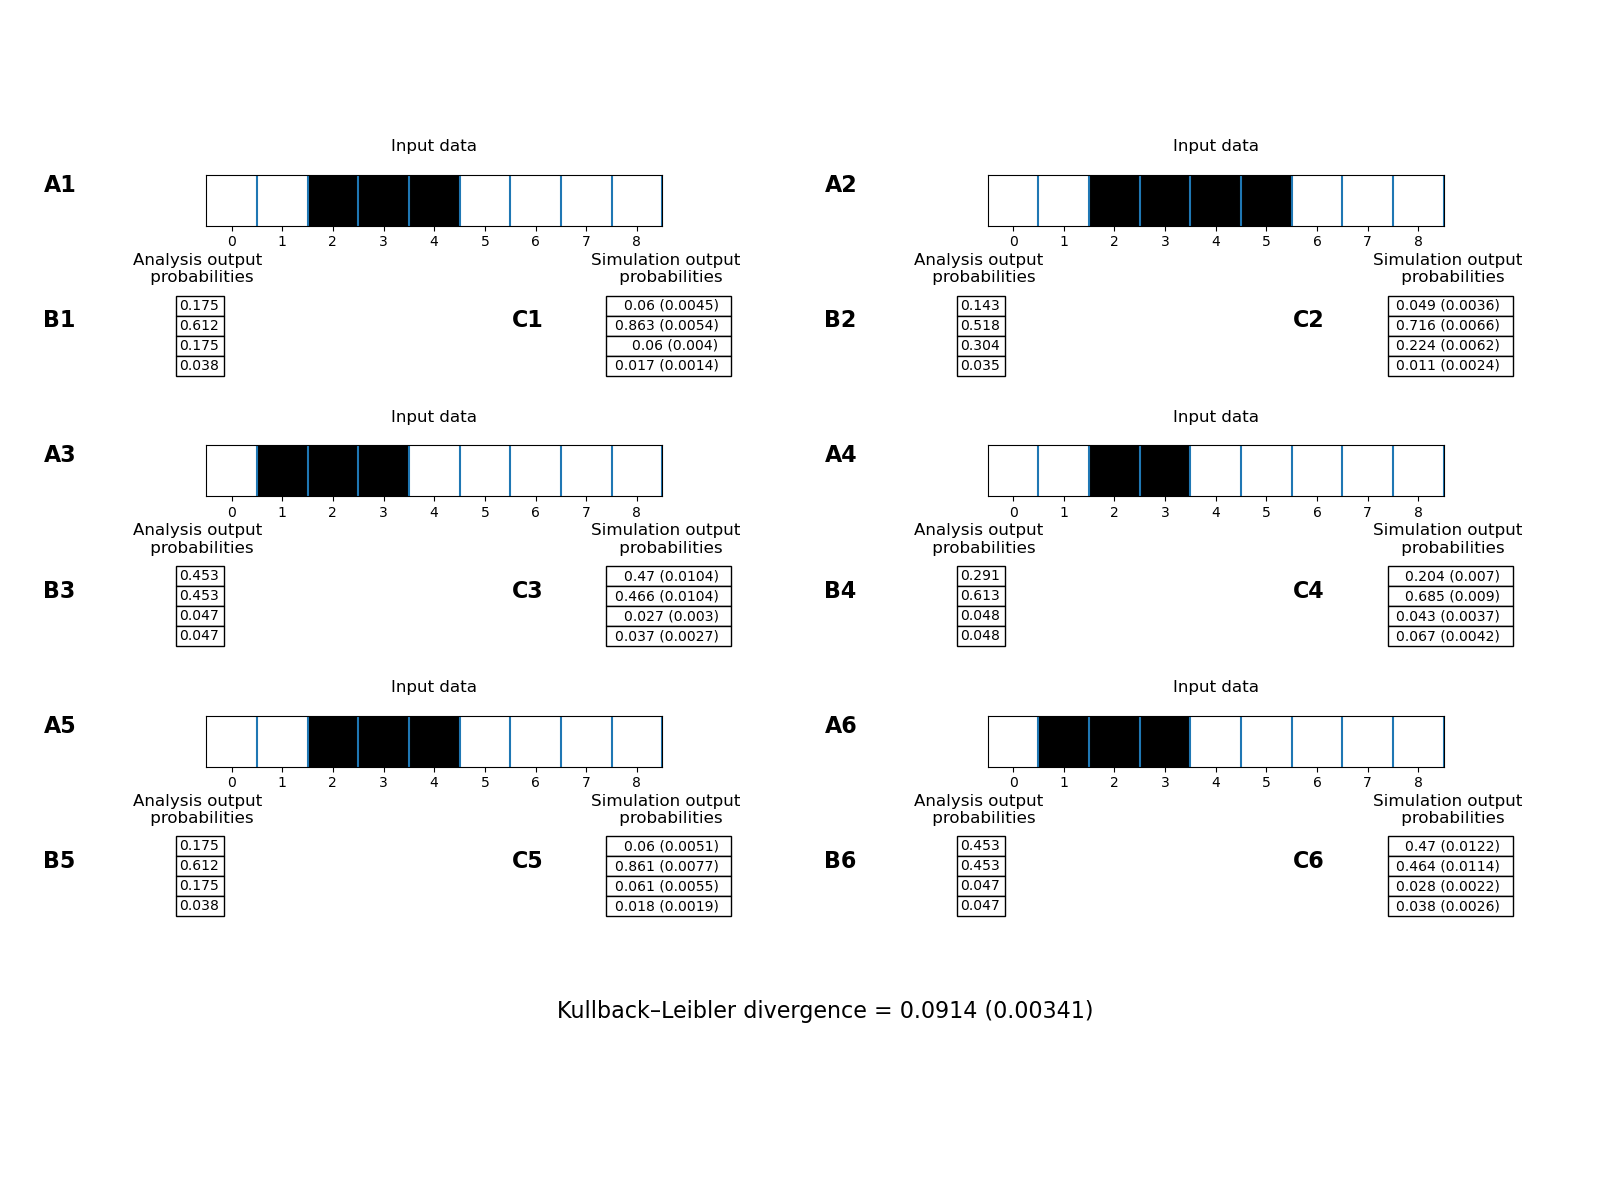
\includegraphics[width=\linewidth]{figures/1D/1D_70_0_15.png}
  \caption{\textbf{Analysis and simulation result. Parameters: }$f_{input} = 70 Hz, f_{prior} = 0 Hz, \tau_{decay} = 15 ms$ \textbf{A} Input images with 9 x 1 pixels. The red borders indicate the class of the prior. \textbf{B} Analytically calculated posterior probabilities. \textbf{C} Proportions of the spikes of the output neurons during the simulation and their standard deviations in brackets.}
  \label{fig:1D_70_0_15}
\end{figure}

\subparagraph{$\tau_{decay} = 0.004 seconds$, $f_{prior} = 0 Hz$}
For this parameter combination values between 50 and 150 Hz for $f_{input}$ in steps of 10 Hz were simulated. Analogously to the previous parameter set after finding the best input firing rate the search was performed in finer steps until the best value was determined as 88 Hz. The result of this search can be seen in Figure \ref{fig:1D_KLD_fPrior0_tau4}. The result of the simulation with those parameters can be seen in Figure \ref{fig:1D_88_0_4}.

\begin{figure}
  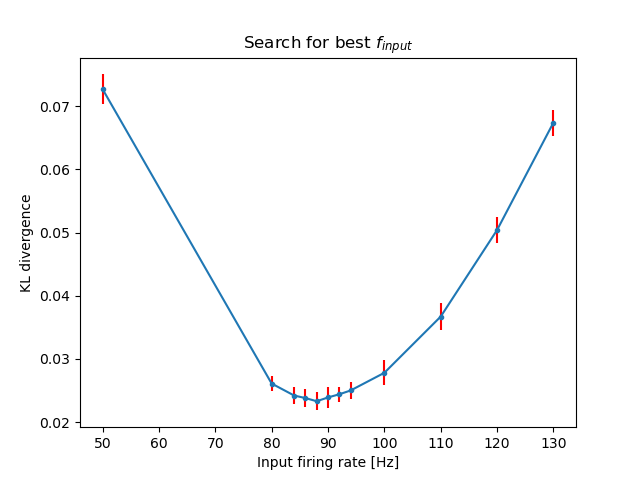
\includegraphics[width=\linewidth]{figures/1D/KLDvsfInput_fPrior0tau4.png}
  \caption{\textbf{KL divergence for different $f_{input} values$} $f_{prior} = 0 Hz, \tau_{decay} = 4 ms$}
  \label{fig:1D_KLD_fPrior0_tau4}
\end{figure}

\begin{figure}
  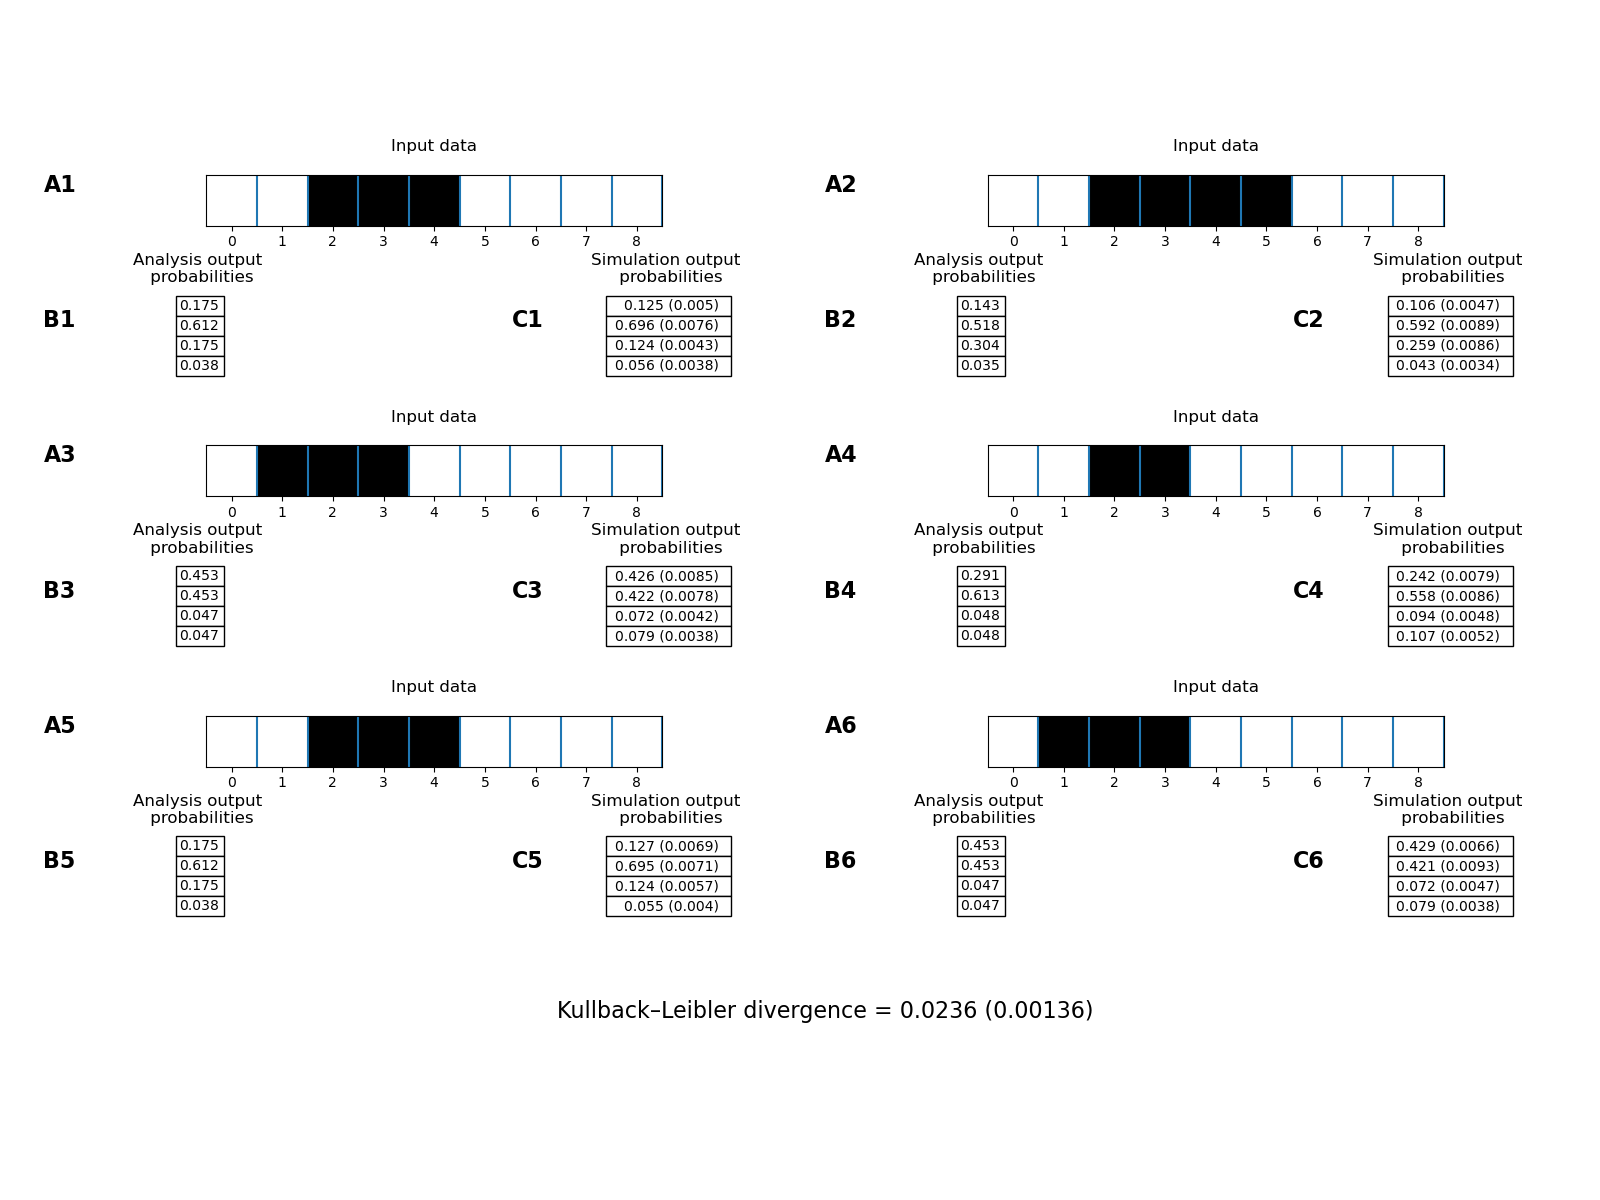
\includegraphics[width=\linewidth]{figures/1D/1D_88_0_4.png}
  \caption{\textbf{Analysis and simulation result. Parameters: } $f_{input} = 88 Hz, f_{prior} = 0 Hz, \tau_{decay} = 4 ms$ \textbf{A} Input images with 9 x 1 pixels. \textbf{B} Analytically calculated posterior probabilities. \textbf{C} Proportions of the spikes of the output neurons during the simulation and their standard deviations in brackets.}
  \label{fig:1D_88_0_4}
\end{figure}

\paragraph{Simulation results with prior}
After determining the best input firing rates for two different values of $\tau_{decay}$, the prior neurons were activated and the best prior firing rate $f_{prior}$ was fitted.
\subparagraph{$\tau_{decay} = 0.015 seconds$, $f_{input} = 42 Hz$}
The search for the best value of $f_{prior}$ was performed in the same manner as for $f_{input}$. Values between 140 and 240 Hz were simulated and a prior firing rate of 222 Hz performed the best. The result of this search can be seen in Figure \ref{fig:1D_KLD_fInput42_tau15}. The simulation results can be seen in Figure \ref{fig:1D_42_222_15}. The value of the prior is indicated by the red border which is three pixels wide and centered at the center position of the corresponding output class.

\begin{figure}
  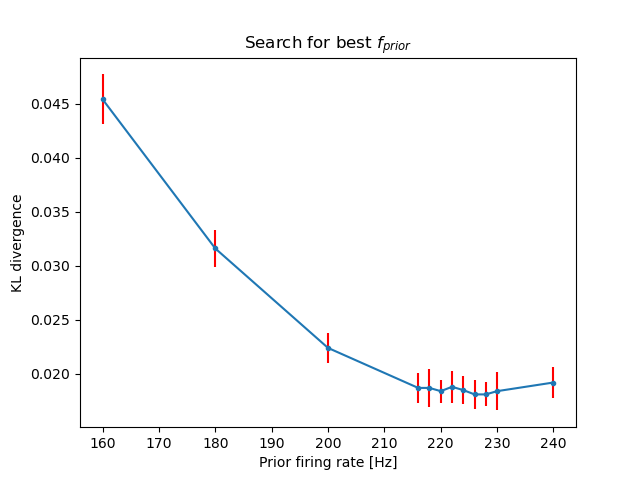
\includegraphics[width=\linewidth]{figures/1D/KLDvsfPrior_fInput42tau15.png}
  \caption{\textbf{KL divergence for different $f_{prior} values$} $f_{input} = 42 Hz, \tau_{decay} = 15 ms$}
  \label{fig:1D_KLD_fInput42_tau15}
\end{figure}

\begin{figure}
  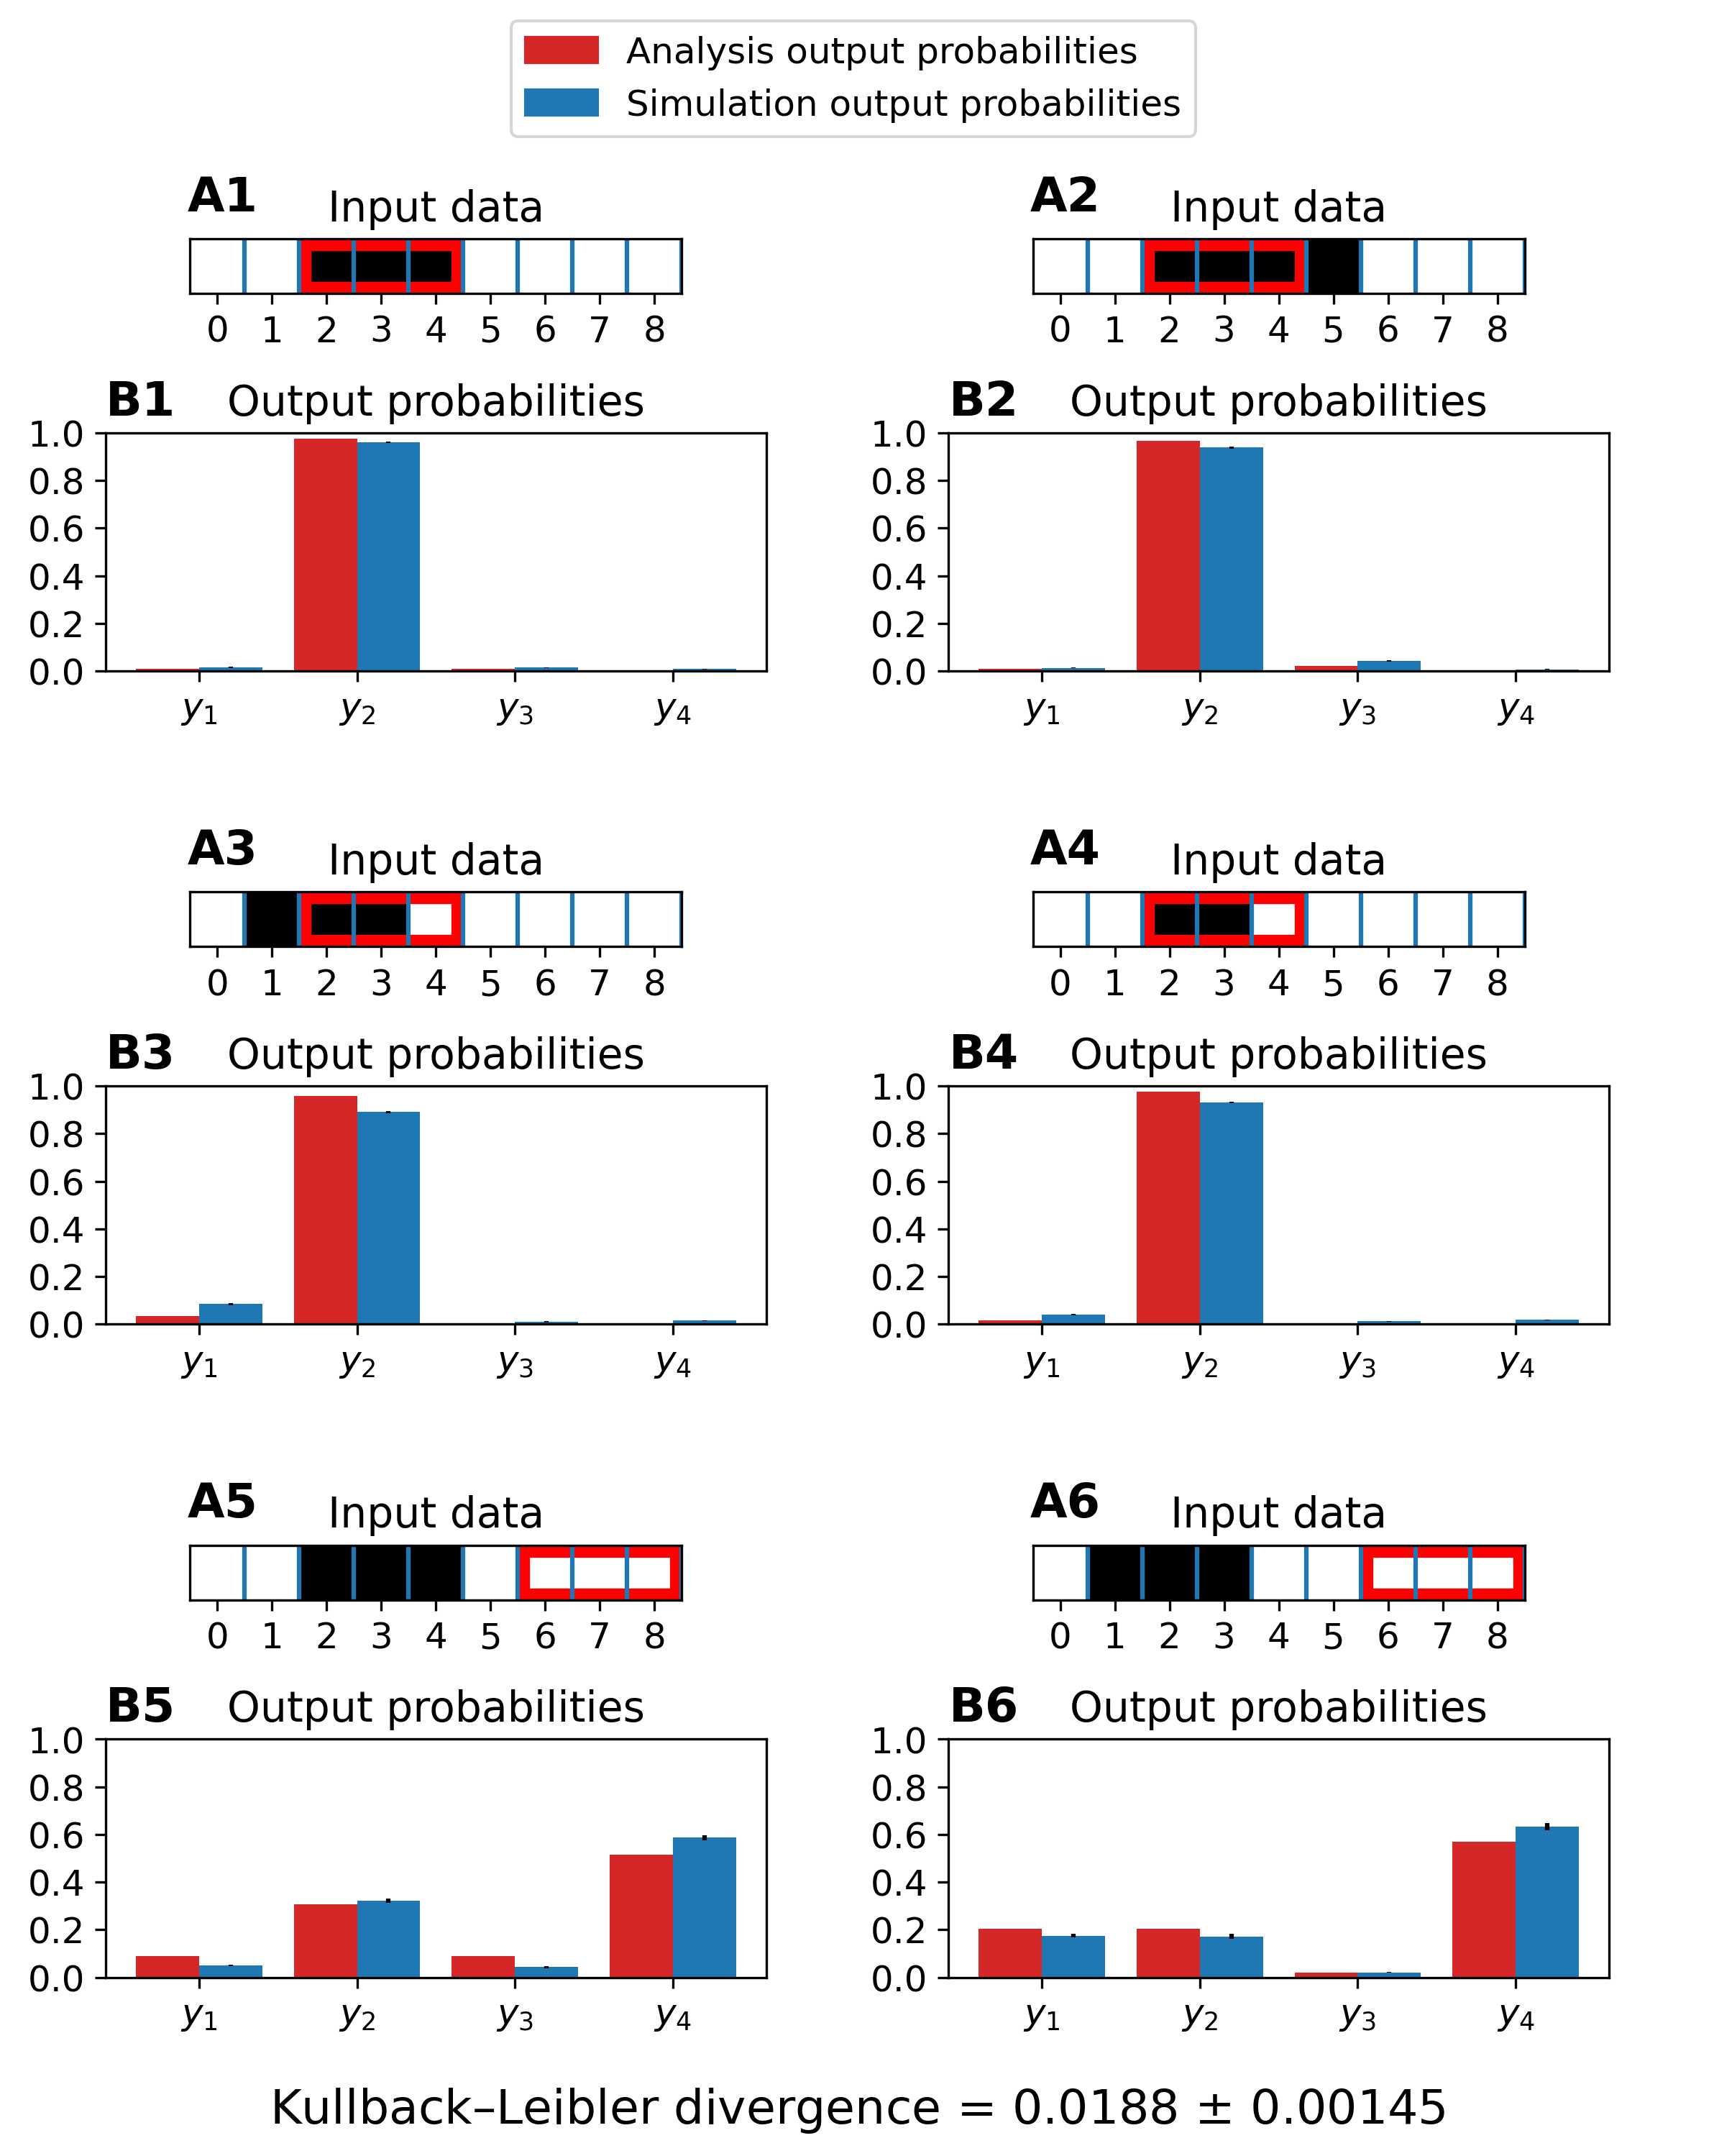
\includegraphics[width=\linewidth]{figures/1D/1D_42_222_15.png}
  \caption{\textbf{Analysis and simulation result. Parameters: } $f_{input} = 42 Hz, f_{prior} = 222 Hz, \tau_{decay} = 15 ms$ \textbf{A} Input images with 9 x 1 pixels. \textbf{B} Analytically calculated posterior probabilities. \textbf{C} Proportions of the spikes of the output neurons during the simulation and their standard deviations in brackets.}
  \label{fig:1D_42_222_15}
\end{figure}

\subparagraph{$\tau_{decay} = 0.004 seconds$, $f_{input} = 88 Hz$}
The search for the best value of $f_{prior}$ was performed in the same manner as for $f_{input}$. Values between 360 and 460 Hz were simulated and a prior firing rate of 440 Hz performed the best. The result of this search can be seen in Figure \ref{fig:1D_KLD_fInput88_tau4}. The results of this parameter combination are given in Figure \ref{fig:1D_88_440_4}.

\begin{figure}
  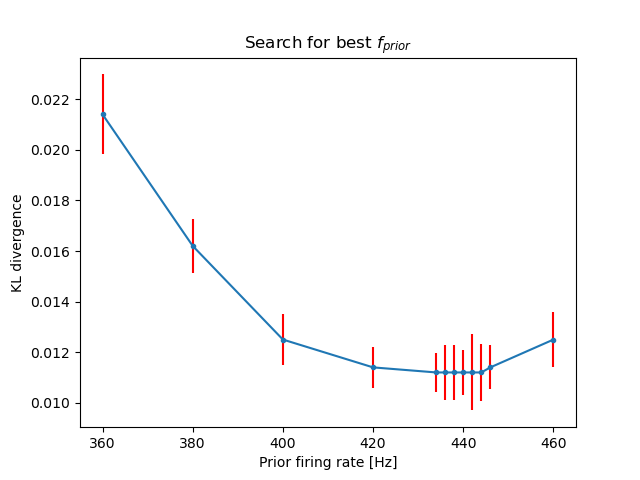
\includegraphics[width=\linewidth]{figures/1D/KLDvsfPrior_fInput88tau4.png}
  \caption{\textbf{KL divergence for different $f_{prior} values$} $f_{input} = 88 Hz, \tau_{decay} = 4 ms$}
  \label{fig:1D_KLD_fInput88_tau4}
\end{figure}

\begin{figure}
  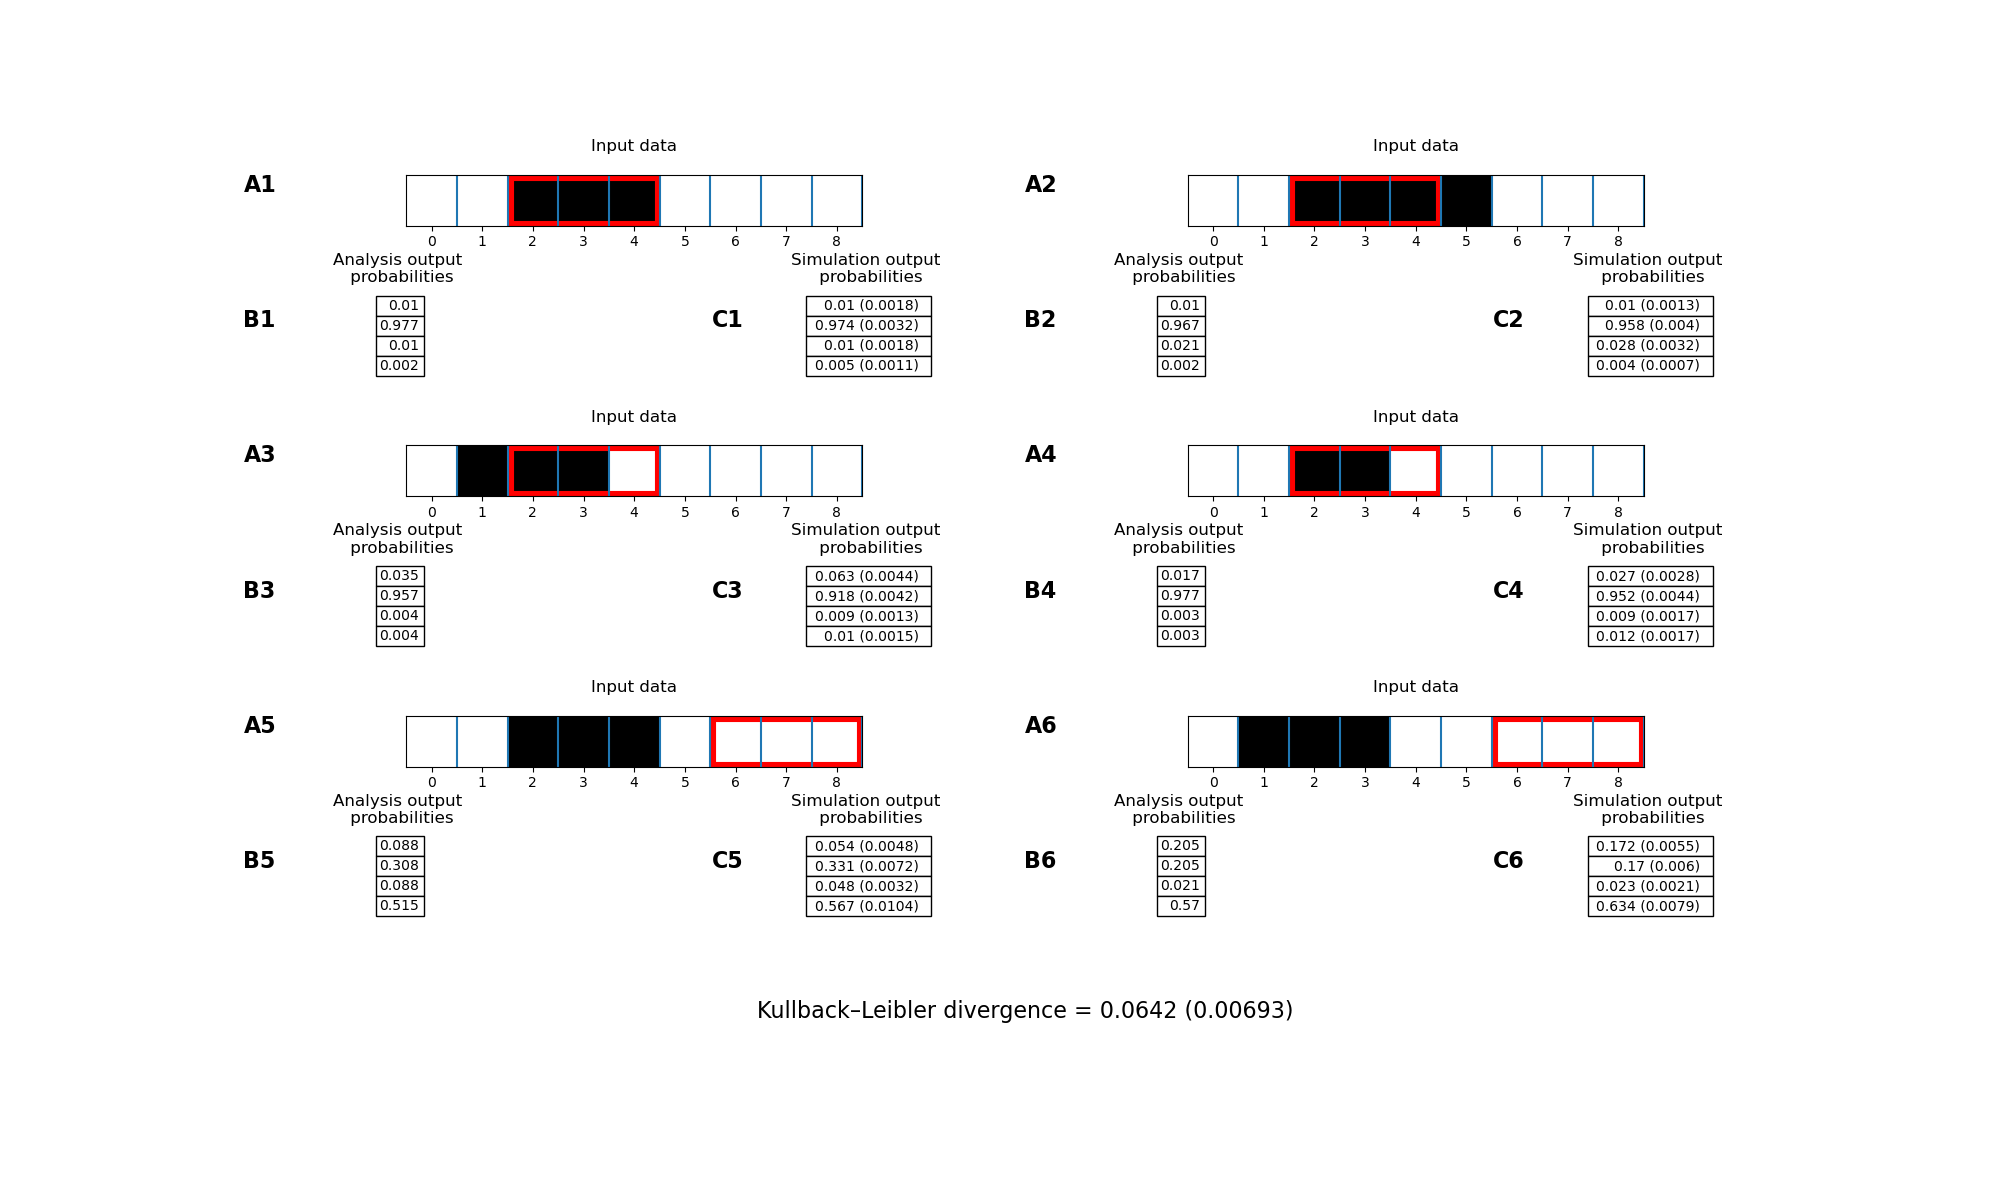
\includegraphics[width=\linewidth]{figures/1D/1D_88_440_4.png}
  \caption{\textbf{Analysis and simulation result. Parameters: } $f_{input} = 88 Hz, f_{prior} = 440 Hz, \tau_{decay} = 4 ms$ \textbf{A} Input images with 9 x 1 pixels. \textbf{B} Analytically calculated posterior probabilities. \textbf{C} Proportions of the spikes of the output neurons during the simulation and their standard deviations in brackets.}
  \label{fig:1D_88_440_4}
\end{figure}

To demonstrate the impact of rising $f_{prior}$ it was set to 600 Hz and the results can be seen in Figure \ref{fig:1D_88_600_4}.

\begin{figure}
  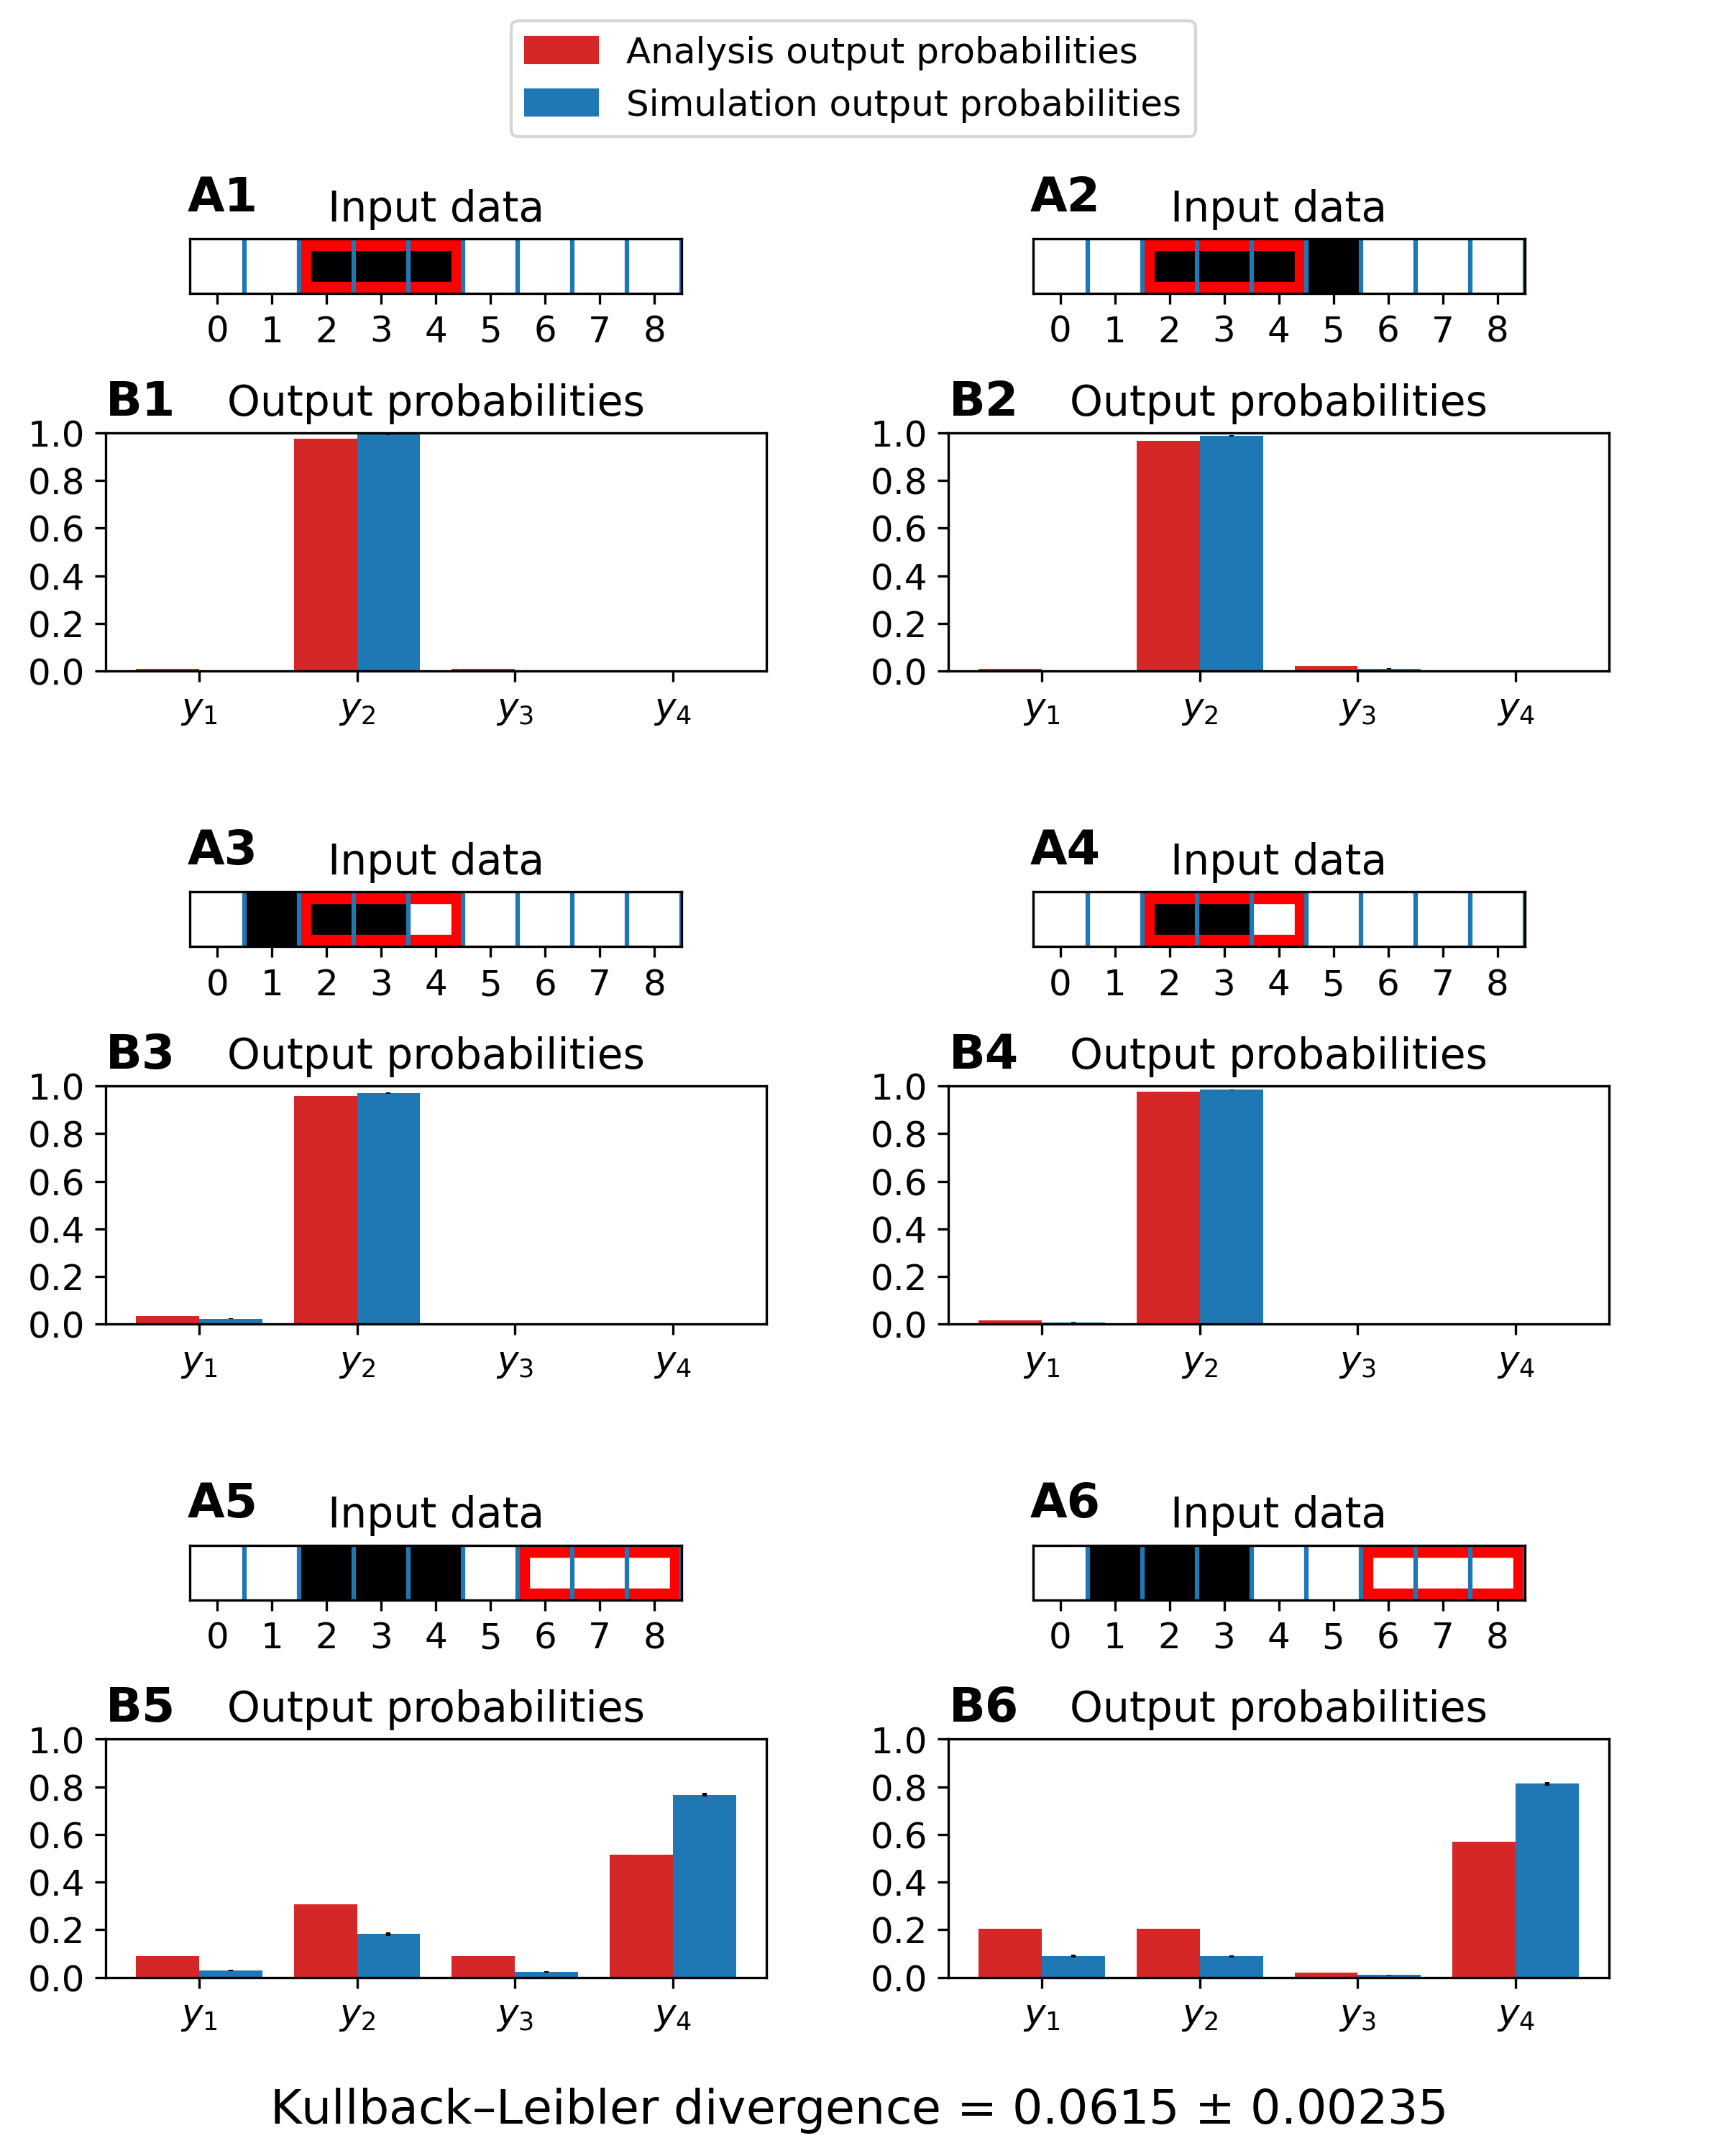
\includegraphics[width=\linewidth]{figures/1D/1D_88_600_4.png}
  \caption{\textbf{Analysis and simulation result. The Kullback-Leibler divergence could not be calculated for this case, as it is not defined for probabilities of 0. Parameters: } $f_{input} = 88 Hz, f_{prior} = 600 Hz, \tau_{decay} = 4 ms$ \textbf{A} Input images with 9 x 1 pixels. \textbf{B} Analytically calculated posterior probabilities. \textbf{C} Proportions of the spikes of the output neurons during the simulation and their standard deviations in brackets.}
  \label{fig:1D_88_600_4}
\end{figure}

\subparagraph{$\tau_{decay} = 0.004 seconds$, $f_{input} = 98$, $f_{prior} = 440 Hz$}
Finally to it was tested if a increase of $f_{input}$ might decrease the Kullback-Leibler divergence even further. The network was simulated with increasing values of $f_{input}$ in steps of 2 Hz, beginning from 90 Hz. The result of this search can be seen in Figure \ref{fig:1D_KLD_fPrior440_tau4}. The best result was obtained with an input firing rate of 98 Hz. The results of that simulation can be seen in Figure \ref{fig:1D_98_440_4}.

\begin{figure}
  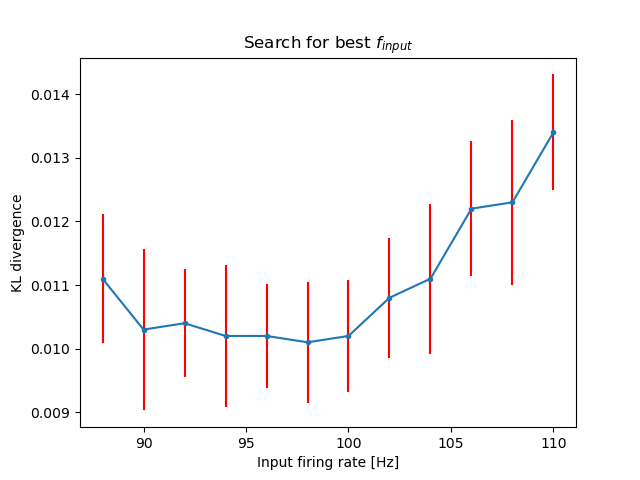
\includegraphics[width=\linewidth]{figures/1D/KLDvsfInput_fPrior440tau4.png}
  \caption{\textbf{KL divergence for different $f_{input} values$} $f_{prior} = 440 Hz, \tau_{decay} = 4 ms$}
  \label{fig:1D_KLD_fPrior440_tau4}
\end{figure}

\begin{figure}
  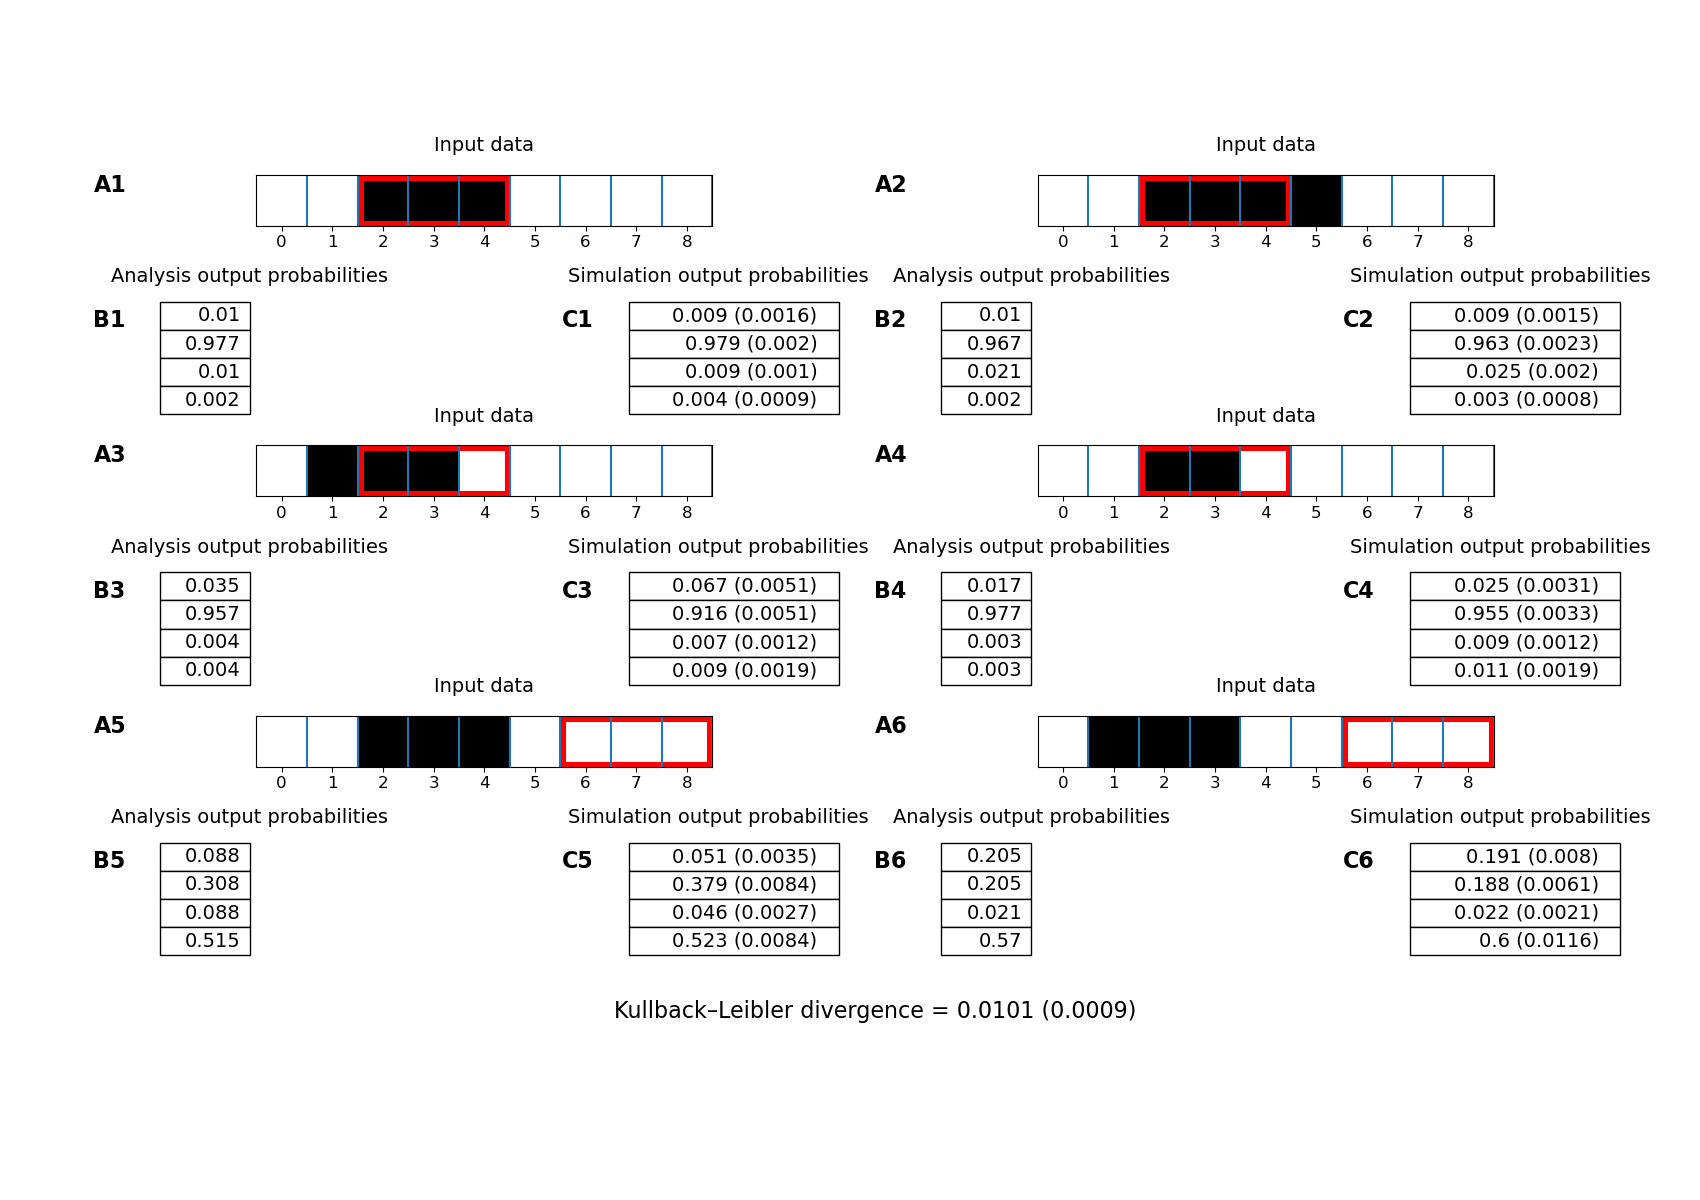
\includegraphics[width=\linewidth]{figures/1D/1D_98_440_4.png}
  \caption{\textbf{Analysis and simulation result. Parameters: } $f_{input} = 98 Hz, f_{prior} = 440 Hz, \tau_{decay} = 4 ms$ \textbf{A} Input images with 9 x 1 pixels. \textbf{B} Analytically calculated posterior probabilities. \textbf{C} Proportions of the spikes of the output neurons during the simulation and their standard deviations in brackets.}
  \label{fig:1D_98_440_4}
\end{figure}

\subsection{Discussion}

In this experiment the impact of the three network parameters $f_{input}$, $f_{prior}$ and $\tau_{decay}$ was analysed.

\paragraph{$f_{input}$} controls how strongly the information of the pixels of the input image is weighed. This means that by raising $f_{input}$ the impact of the active pixels increases, while the impact of the prior neuron decreases comparatively. This effect will be shown in the discussion about $f_{prior}$. However this is not the only impact this parameter has. When raising $f_{input}$ it was also observed that the probabilities for output classes adjacent to the active pixels decreased. This can be observed when comparing Figures \ref{fig:1D_42_0_15} and \ref{fig:1D_70_0_15} where $f_{input}$ was raised from 42 Hz to 70 Hz. For example when looking at "C4" in the mentioned figures, it can be seen that for $f_{input} = 42 Hz$ the simulation output probability for class 1 is 0.245. This high probability is mostly due to the active pixel number 2, which belongs to class 1 and 2 at the same time. When now increasing $f_{input}$ to 70 Hz one might expect the probabilities for class 1 and 2 to rise. This however does not happen, instead the simulation output probability for class 1 fell to 0.207, while for class 2 it rose.
It is assumed that this happens because the membrane potentials of the output neurons are never normalized. As the input neurons spike more quickly the membrane potential of output neuron 1 rises slower than the membrane potential of output neuron 2. This leads to shifted firing rates in favour of output neuron 2. However this behaviour might be expected, as faster spiking input neurons correspond statistically to taking more samples of a probability distribution. This means that the more samples the network takes, the more certain it becomes of the more likely option, which is output class 2.

\paragraph{$f_{prior}$} When increasing the prior firing rate the impact on the result of the prior neurons increases, while the impact of the input neurons decreases comparatively. When comparing the Figures \ref{fig:1D_88_440_4} and \ref{fig:1D_88_600_4} which show the results for $f_{input} = 88 Hz$, $\tau_{decay} = 4 ms$ and $f_{prior} = 440$ and $600 Hz$ respectively it can be seen under "C6" how the probability for output class 4 rose, while all other probabilities fell. The opposite behaviour can be observed when raising $f_{input}$ instead, but no separate figure will be provided for this case.

\paragraph{$\tau_{decay}$} determines for how long and how strongly an input or prior spike contributes to the membrane potentials of the output neurons. The bigger $\tau_{decay}$ is, the smaller $f_{input}$ and $f_{prior}$ need to be, to minimize the Kullback-Leibler divergence. This is represented by the final parameters for $\tau_{decay}$ of 4 and 15 ms. While for $\tau_{decay} = 15 ms$ the best input firing rate was 42 Hz and the prior firing rate was 222 Hz, for $\tau_{decay} = 4 ms$ they had to be raised to 98 and 440 Hz to minimize the Kullback-Leibler divergence.

\paragraph{Approximating the analytic solution}
After first finding the optimal $f_{input}$ for disabled prior activity and then finding the optimal $f_{prior}$ with enabled prior activity for $\tau_{decay}$ the simulation was not yet approximating the analytical solution perfectly. Because of that it was tried to raise $f_{input}$ to further decrease the Kullback-Leibler divergence. The further search for a better $f_{input}$ was performed for $\tau_{decay} = 0.004 ms$ and $f_{prior} = 440 Hz$, as this set of parameters performed the best overall.
When comparing the former optimal result in Figure \ref{fig:1D_88_440_4} with $f_{input} = 88 Hz$, to the result with $f_{input} = 98 Hz$ in Figure \ref{fig:1D_98_440_4}, it can be seen that the Kullback-Leibler divergence decreased from 0.0112 to 0.0101. The simulation output probabilities with the higher $f_{input}$ approximated the analysis output probabilities for example for "B3" and "C3" in the mentioned figures on one hand better, while on the other hand for "B5" and "C5" the output probabilities of the analysis and the simulation of class 2 diverged more. A further increase of $f_{input}$ started to increase the Kullback-Leibler divergence again, thus the final optimum of the parameter set was reached. It is assumed that increasing $f_{input}$ after $f_{prior}$ was fitted was necessary because the proportion of the impact of $f_{input}$ on the simulation decreased due to the introduction of the prior activity.

\section{Experiment 6: Simulation of the 1D network with double size}
\label{section:1DDoubleSize}

\subsection{Introduction}
In this experiment the optimal parameters determined in Experiment 5 were used for a network double in size of the network in Experiment 5. By doing this the applicability of parameters determined for one network to another network was to be examined.

\subsection{Methods}
The network of Experiment 5 was doubled in size by increasing the number of input neurons from 18 to 36 neurons. This resulted in input images with 18 pixels. Furthermore the matrix $P^{X|Y}$ was doubled in size by inserting each value of the matrix to the right of itself. The amount of the prior neurons was kept the same with 4 prior neurons. However this network was simulated once for a prior firing rate of 440 Hz, and once for the double rate of 880 Hz. The rest of the methods were performed analogously to Experiment 5.

\subsection{Results}

The expanded matrix $P^{X|Y}$ was doubled in size, now being $[18 \times 4]$ yielding
\begin{equation}
\label{eqn:pXvorausgesetztYResultDoubled}
P^{X|Y} = \begin{bmatrix}
0.9 & 0.9 & 0.9 & 0.9 & 0.9 & 0.9 & 0.1 & 0.1 & 0.1 & ...\\
... & 0.1 & 0.9 & 0.9 & 0.9 & 0.9 & 0.9 & 0.9 & 0.1 & ...\\
... & 0.1 & 0.9 & 0.9 & 0.9 & 0.9 & 0.9 & 0.9 & 0.1 & ...\\
... & 0.1 & 0.1 & 0.1 & 0.9 & 0.9 & 0.9 & 0.9 & 0.9 & 0.9\\
\end{bmatrix}.
\end{equation}

The simulation result for $f_{input} = 98 Hz$, $f_{prior} = 440 Hz$ and $\tau_{decay} = 4 ms$ can be seen in Figure \ref{fig:doubleSize_98_440_4}. The Kullback-Leibler divergence is infinity in this result, because some simulation output probabilities were zero and the Kullback-Leibler divergence is not defined for probabilities of zero. To circumvent this an approximated Kullback-Leibler divergence was calculated by setting the simulation output probabilities that were 0 to 0.0000001. This yielded a Kullback-Leibler divergence of 0.1411.
\begin{figure}
  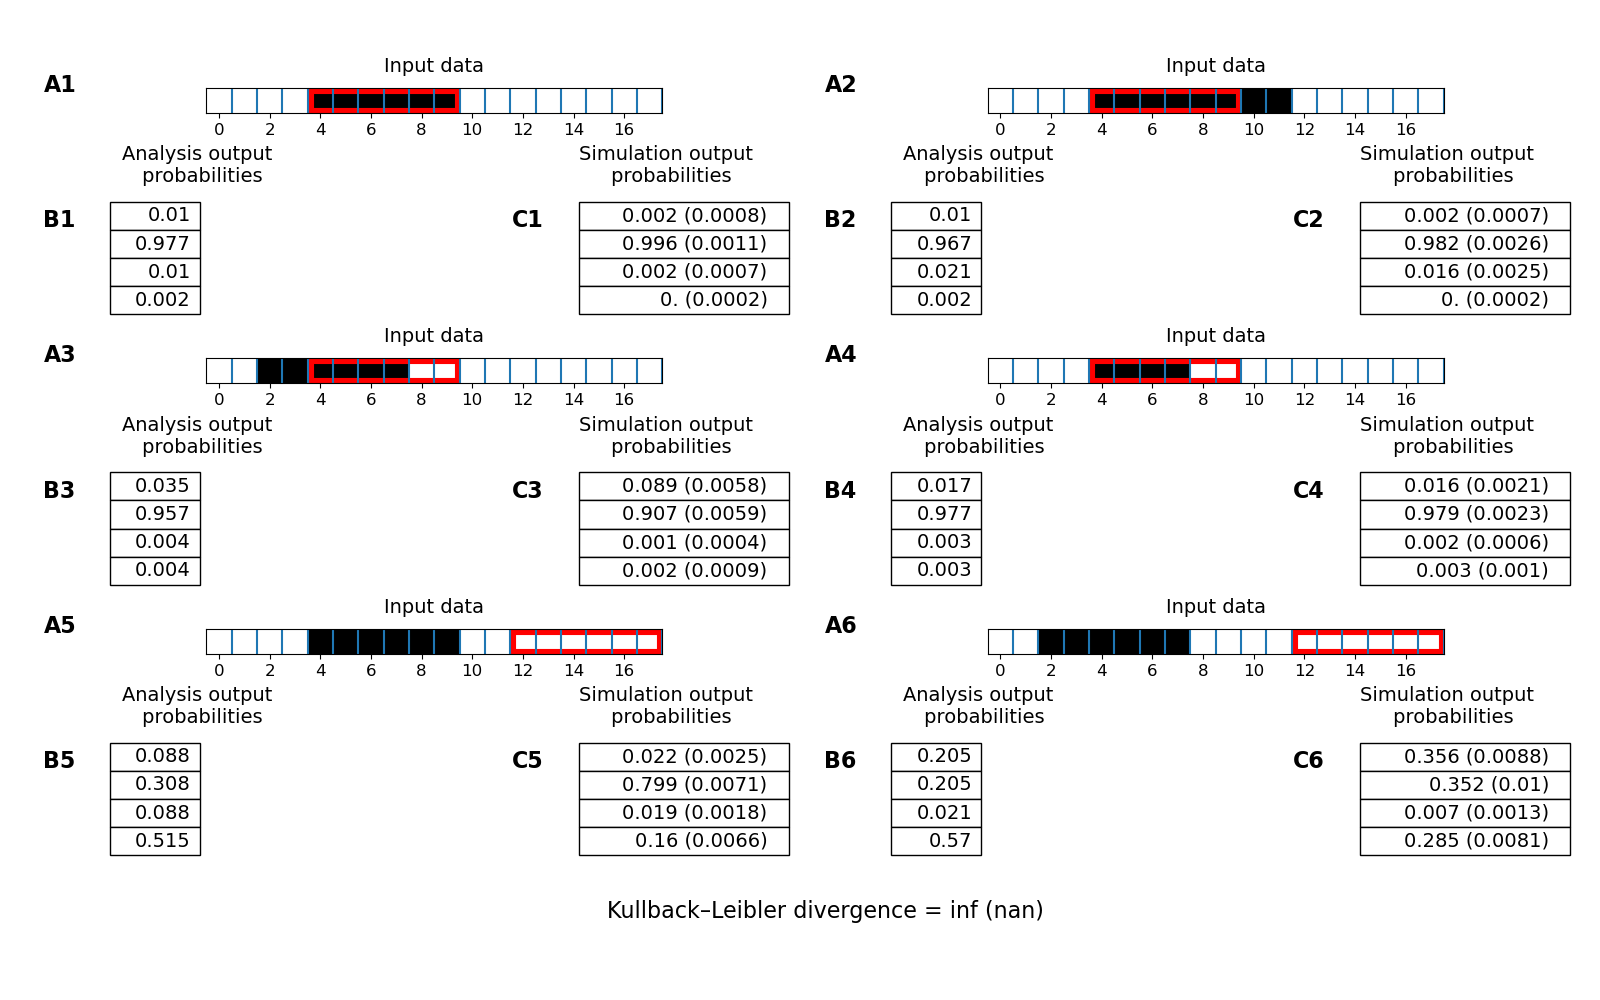
\includegraphics[width=\linewidth]{figures/1D/doubleSize/doubleSize_98_440_4.png}
  \caption{\textbf{Analysis and simulation result. Parameters: } $f_{input} = 98 Hz, f_{prior} = 440 Hz, \tau_{decay} = 4 ms$ \textbf{A} Input images with 18 x 1 pixels. \textbf{B} Analytically calculated posterior probabilities. \textbf{C} Proportions of the spikes of the output neurons during the simulation and their standard deviations in brackets.}
  \label{fig:doubleSize_98_440_4}
\end{figure}

Finally the simulation result for $f_{input} = 98 Hz$, $f_{prior} = 880 Hz$ and $\tau_{decay} = 4 ms$ can be seen in Figure \ref{fig:doubleSize_98_880_4}. As in the previous result the Kullback-Leibler divergence was approximated and calculated as 0.2391 for this parameter set.
\begin{figure}
  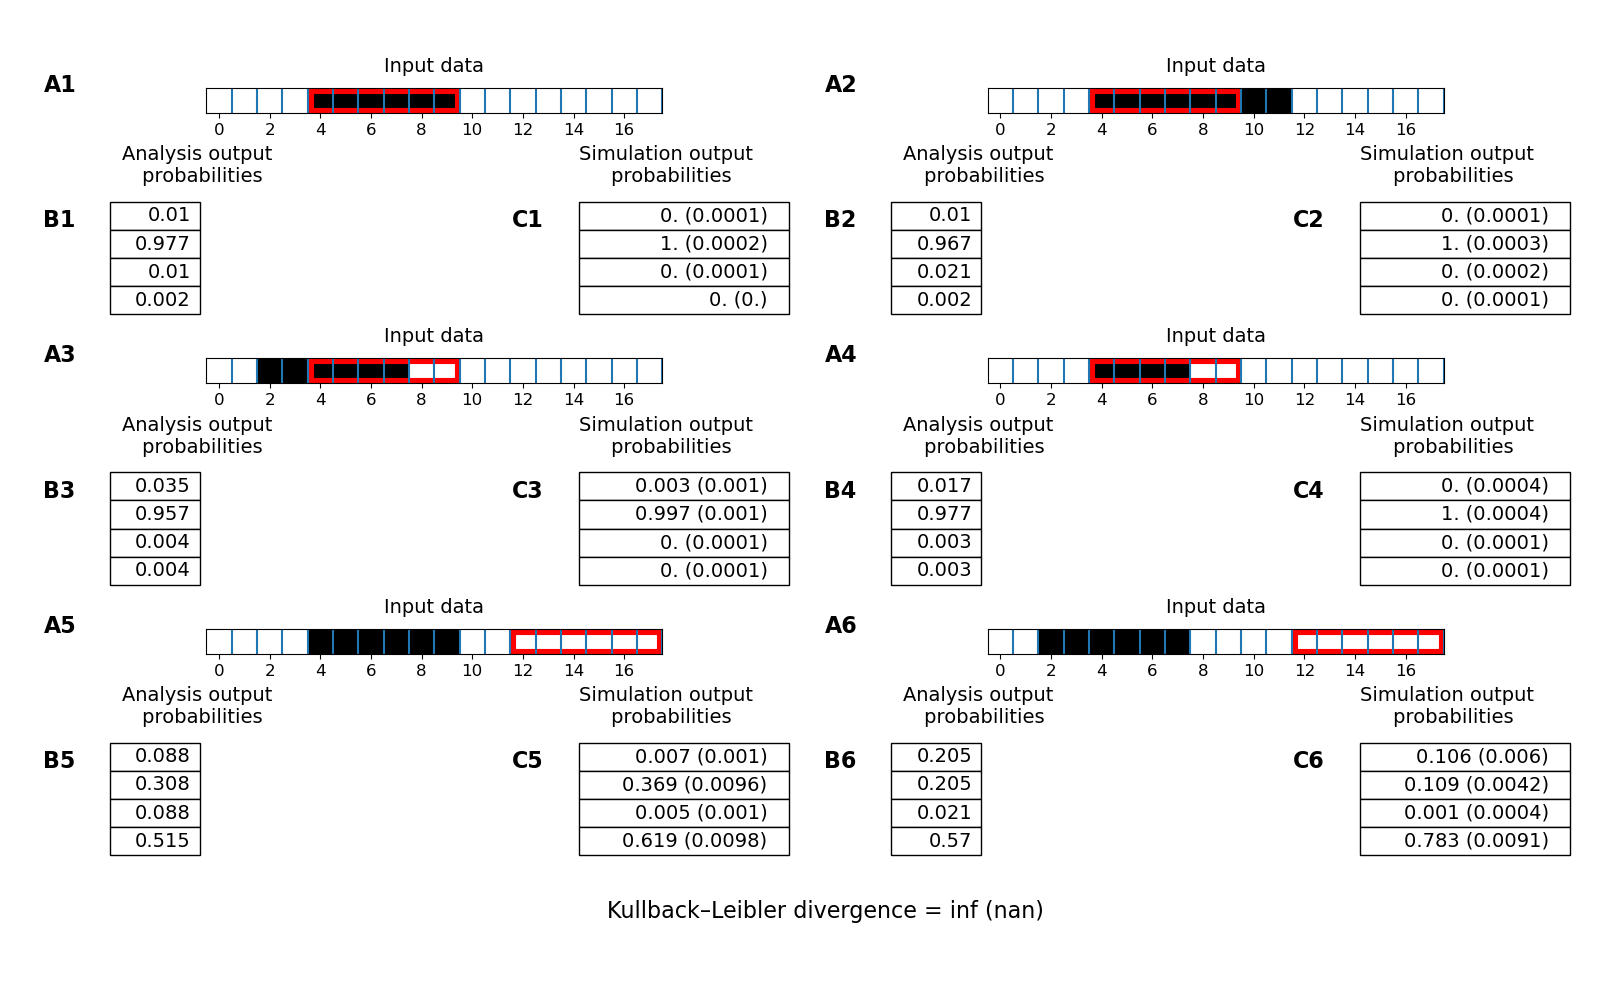
\includegraphics[width=\linewidth]{figures/1D/doubleSize/doubleSize_98_880_4.png}
  \caption{\textbf{Analysis and simulation result. Parameters: } $f_{input} = 98 Hz, f_{prior} = 880 Hz, \tau_{decay} = 4 ms$ \textbf{A} Input images with 18 x 1 pixels. \textbf{B} Analytically calculated posterior probabilities. \textbf{C} Proportions of the spikes of the output neurons during the simulation and their standard deviations in brackets.}
  \label{fig:doubleSize_98_880_4}
\end{figure}

Finally the Kullback-Leibler divergence for the results of the network in Experiment 5 with the parameters $f_{input} = 98 Hz$, $f_{prior} = 440 Hz$ and $\tau_{decay} = 4 ms$ was also approximated in the above mentioned way and resulted in a value of 0.0094.

\subsection{Discussion}

When comparing Figures \ref{fig:1D_98_440_4} and \ref{fig:doubleSize_98_440_4} it can be seen that the analysis output probabilities stayed the same. This is expected, because by doubling the pixels of the input images the information within it does not change as the areas corresponding to an output class double in size, as do the active pixels shown in black. However when comparing the Kullback-Leibler divergences of the network in Experiment 5 and the network of this experiment with parameters of $f_{input} = 98 Hz$, $f_{prior} = 440 Hz$ and $\tau_{decay} = 4 ms$ it can be seen the the network with double size performed worse. The Kullback-Leibler divergence of the network with doubled size was 0.1411 compared to 0.0094 of the network the parameters were fitted to. This clearly indicates that the fitted parameters are not universal to every network size. This might be due to the fact that the membrane potentials of the output neurons are never normalized, which was already discussed in Experiment 5. However if such a normalization was implemented the fitted parameters of one network size could be universal to all other sizes.

\section{Experiment 7: Training of the 1D network with predetermined parameters}
\label{section:1DPreDetermined}

\subsection{Introduction}

In this Experiment the network of Experiment 5 was used, but the weights of the network were not derived from the matrices $P^{X|Y}$ and $P^{Y|Z}$, but they were learned from the input images.

\subsection{Methods}

The network architecture was the same as in Experiment 5 and the training paradigm was the same as in Experiment 4. The used network parameters were $f_{input} = 98 Hz$, $f_{prior} = 440 Hz$ and $\tau_{decay} = 4 ms$. First the weight shifting parameter c was set to 1. Additionally to improve the results the values 2, 3 and 4 were also tried for c.

\subsection{Results}

The training results can be seen in Figure \ref{fig:1DTraining}. 
\begin{figure}
  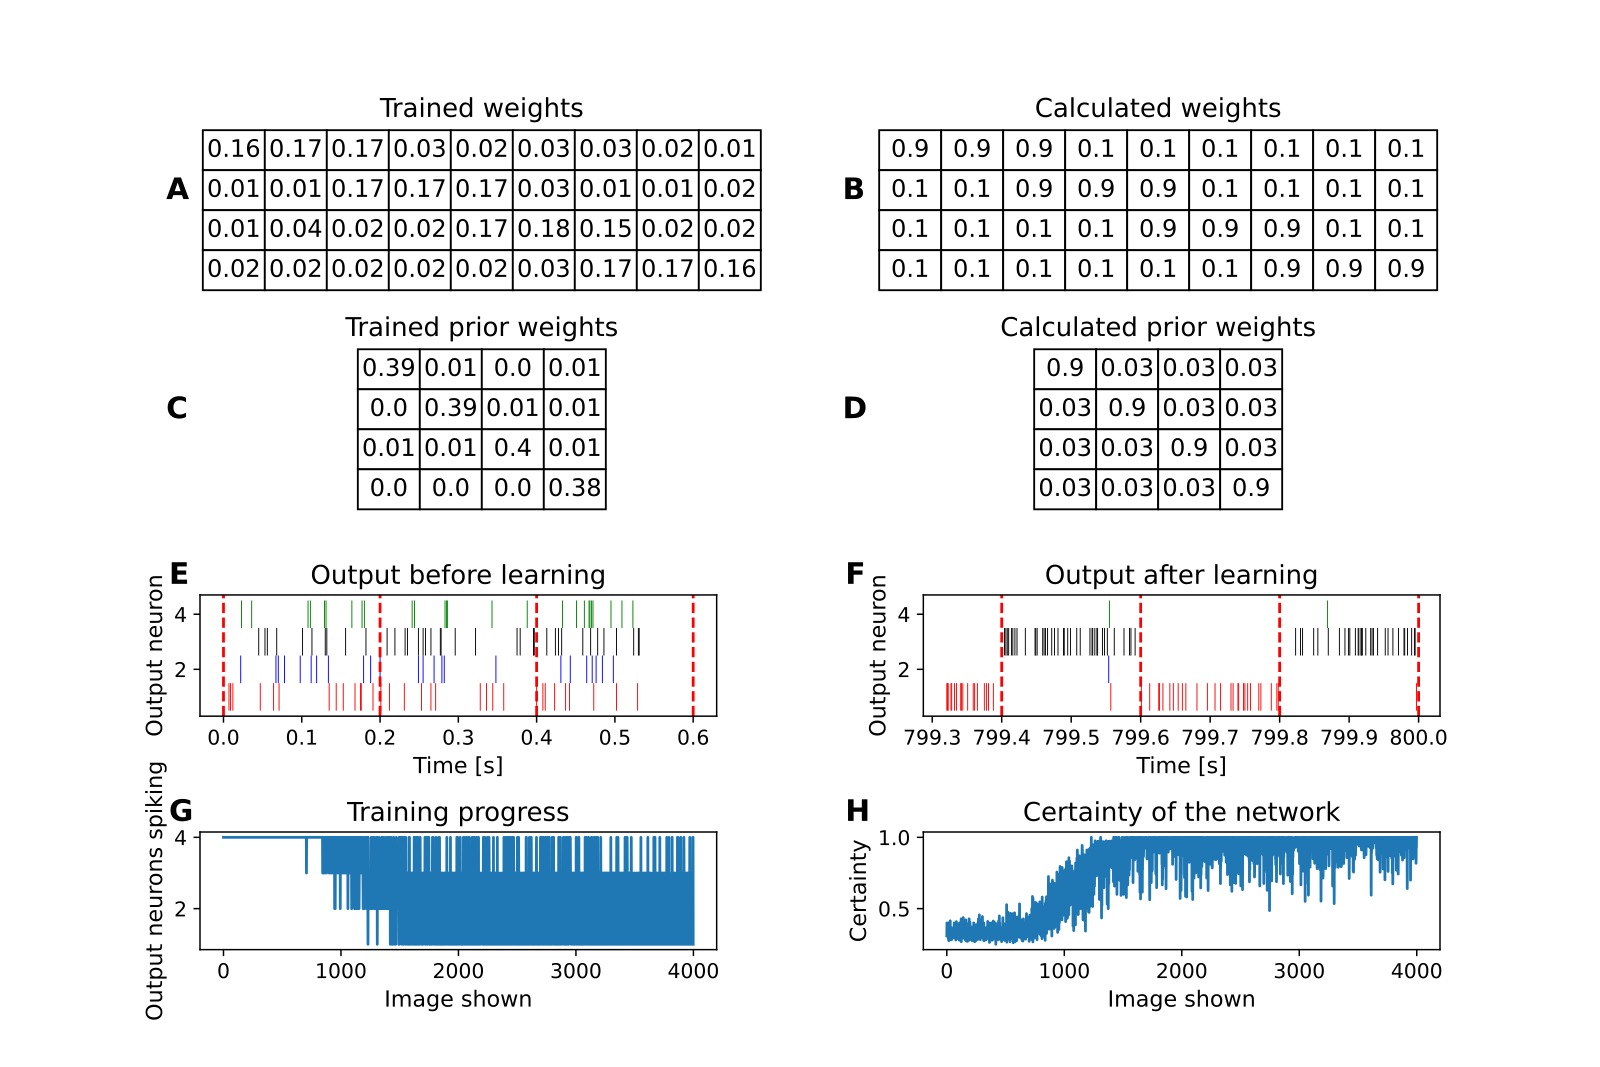
\includegraphics[width=\linewidth]{figures/1D/training/trainingPlot_98_440_4.png}
  \caption{\textbf{Training result} $f_{input} = 98 Hz, f_{prior} = 440 Hz, \tau_{decay} = 4 ms, c = 1$ \textbf{A} The learned probability matrix $P^{X|Y}$. It was determined by taking the weights to the power of e. \textbf{B} The calculated probability matrix $P^{X|Y}$. \textbf{C} The learned prior probability matrix $P^{Y|Z}$. \textbf{D} The calculated prior probability matrix $P^{Y|Z}$. \textbf{E, F} Spike activity expressed by the output neurons before and after the training of the network. \textbf{G} Number of distinct output neurons active during the presentation duration of each training image. \textbf{H} Proportion of most active output neuron  to activity of all other output neurons during the presentation duration of each training image.}
  \label{fig:1DTraining}
\end{figure}

The evaluation results can be seen in Figure \ref{fig:1DTrainingEvaluation}.
\begin{figure}
  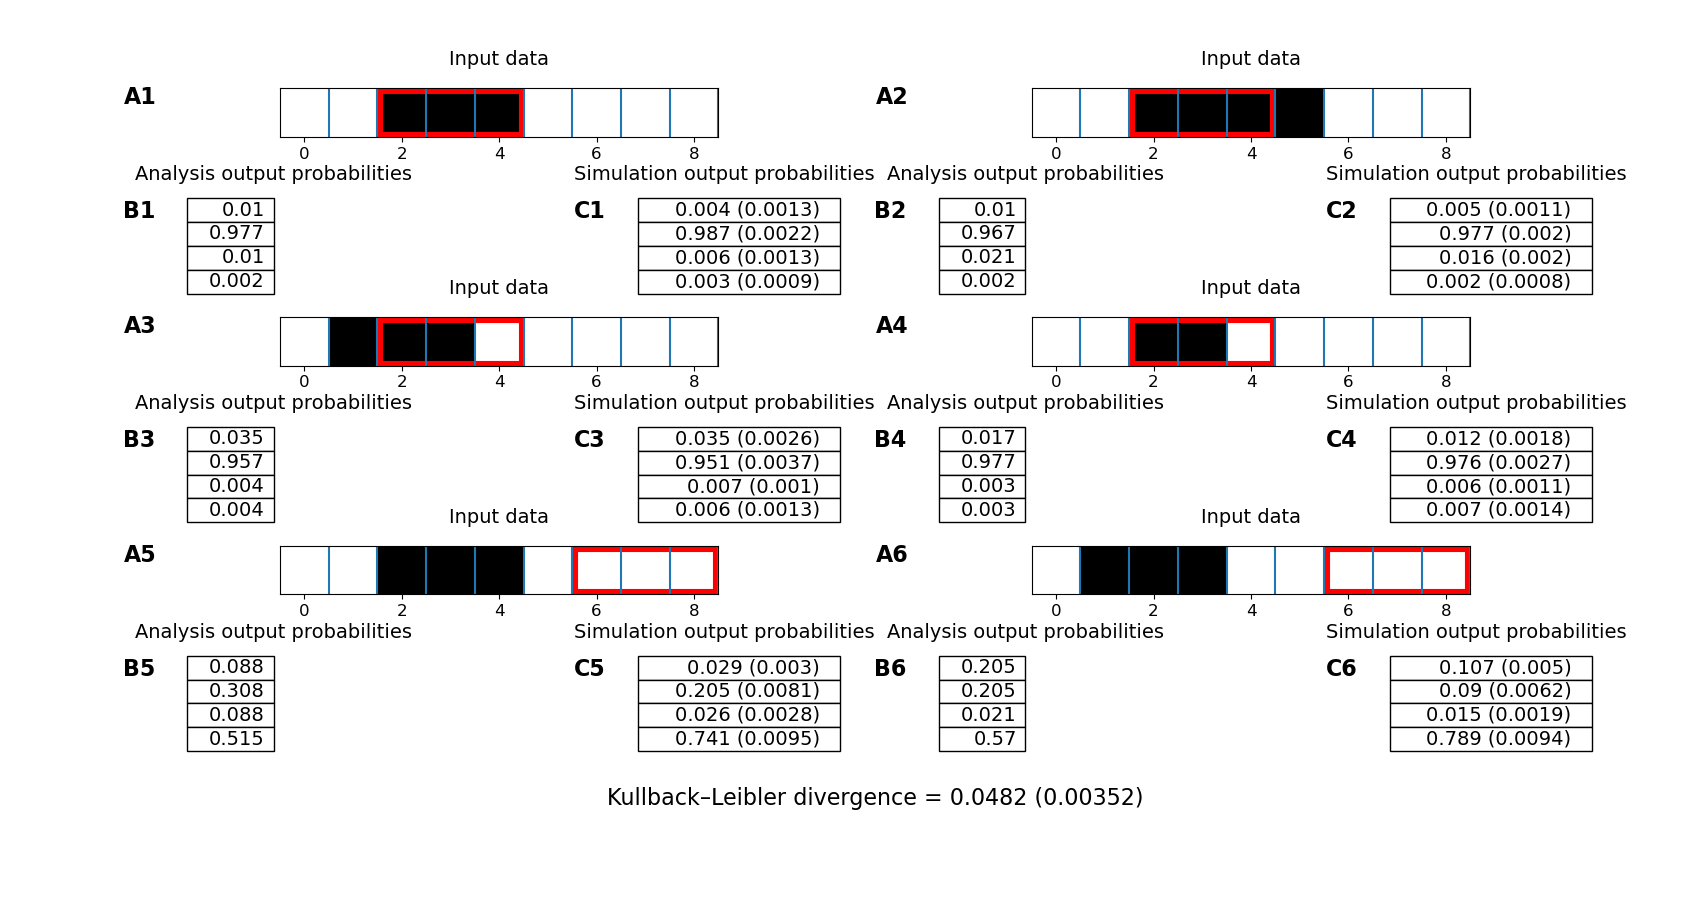
\includegraphics[width=\linewidth]{figures/1D/training/trainingEvaluation_98_440_4.png}
  \caption{\textbf{Analysis and simulation result. Parameters: } $f_{input} = 98 Hz, f_{prior} = 440 Hz, \tau_{decay} = 4 ms$ \textbf{A} Input images with 9 x 1 pixels. \textbf{B} Analytically calculated posterior probabilities. \textbf{C} Proportions of the spikes of the output neurons during the simulation and their standard deviations in brackets.}
  \label{fig:1DTrainingEvaluation}
\end{figure}

The Kullback-Leibler divergence for different values of c can be seen in Figure \ref{fig:1DTrainingC}.
\begin{figure}
  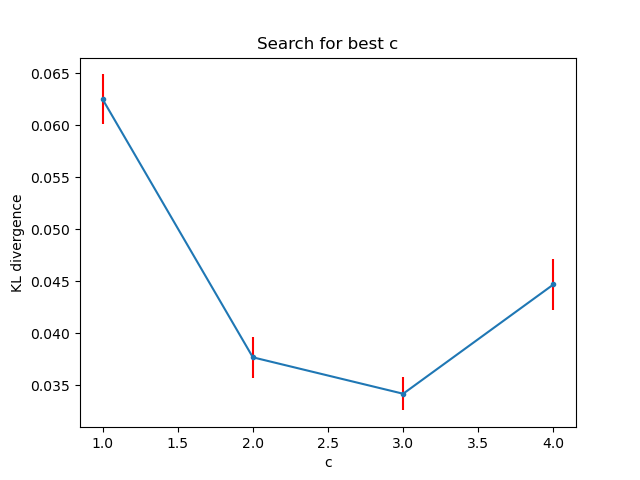
\includegraphics[width=\linewidth]{figures/1D/training/KLD_cvsfInput98_fPrior440tau4.png}
  \caption{\textbf{KL divergence for different c values} $f_{input} = 98 Hz, f_{prior} = 440 Hz, \tau_{decay} = 4 ms$}
  \label{fig:1DTrainingC}
\end{figure}

The training and evaluation results for the best value of $c = 3$ can be seen in Figures \ref{fig:1DTrainingC3} and \ref{fig:1DTrainingEvaluationC3}.

\begin{figure}
  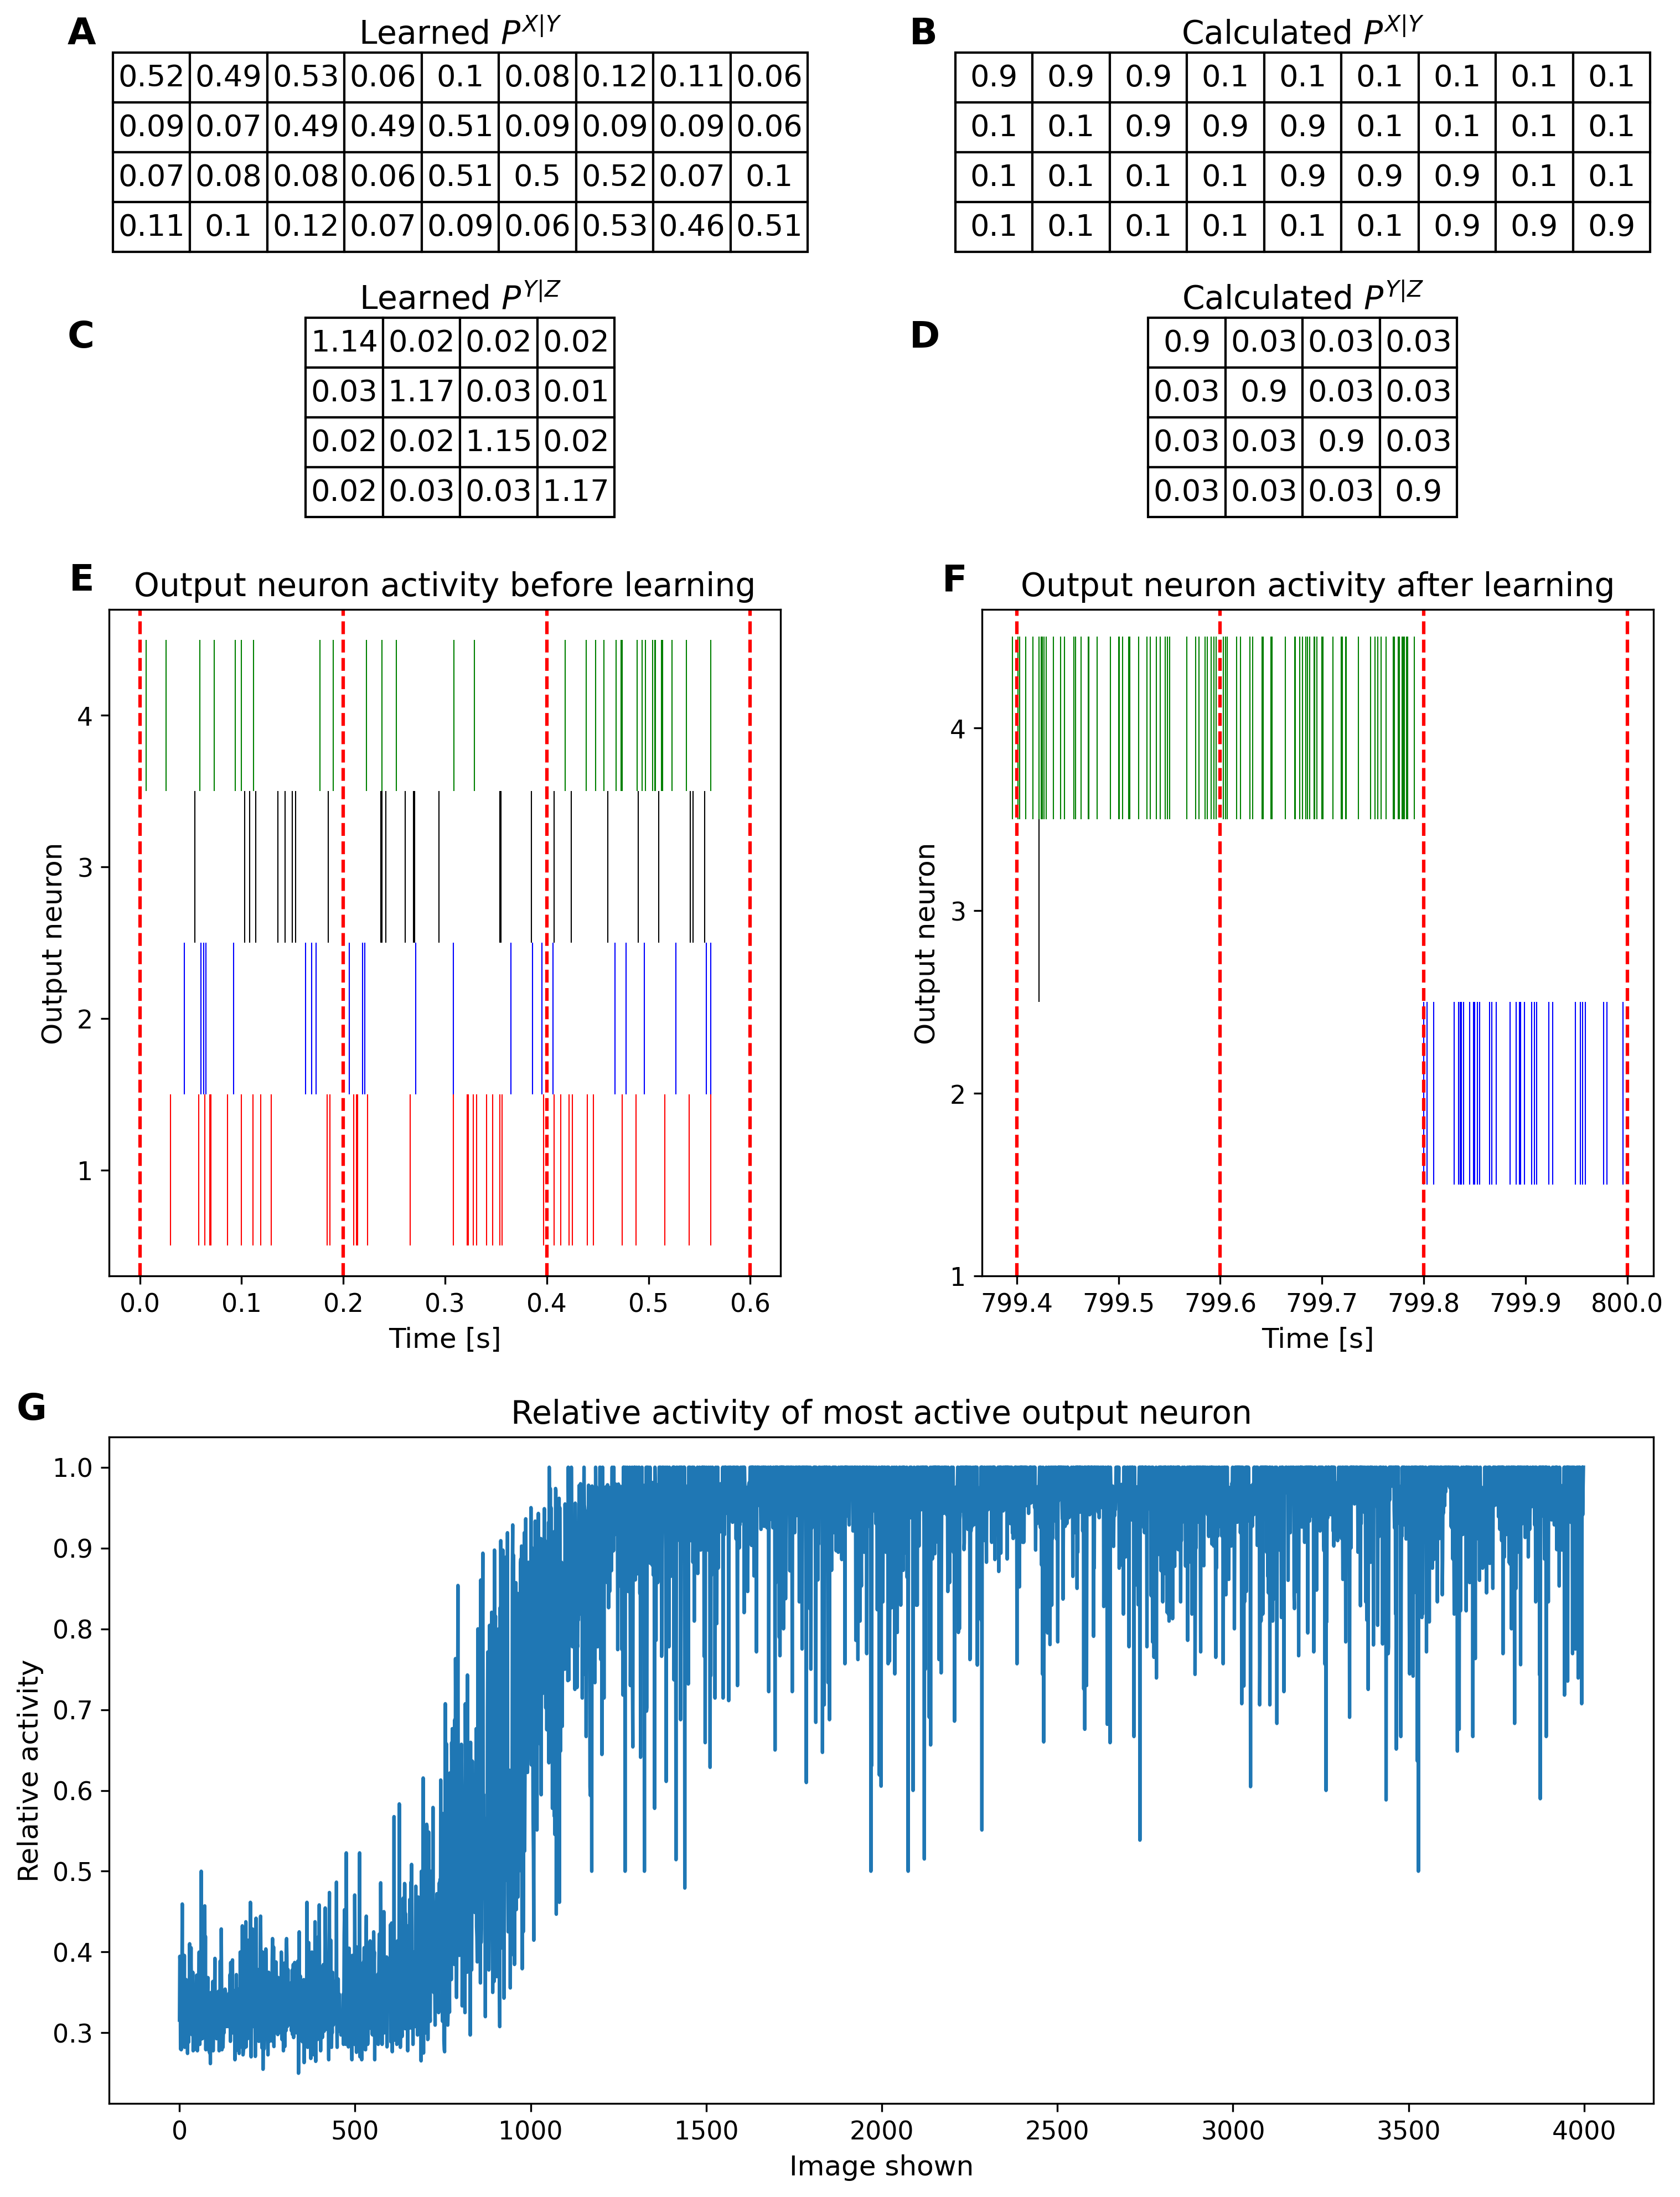
\includegraphics[width=\linewidth]{figures/1D/training/trainingPlot_98_440_4_c3.png}
  \caption{\textbf{Training result} $f_{input} = 98 Hz, f_{prior} = 440 Hz, \tau_{decay} = 4 ms, c = 3$ \textbf{A} The learned probability matrix $P^{X|Y}$. It was determined by taking the weights to the power of e. \textbf{B} The calculated probability matrix $P^{X|Y}$. \textbf{C} The learned prior probability matrix $P^{Y|Z}$. \textbf{D} The calculated prior probability matrix $P^{Y|Z}$. \textbf{E, F} Spike activity expressed by the output neurons before and after the training of the network. \textbf{G} Number of distinct output neurons active during the presentation duration of each training image. \textbf{H} Proportion of most active output neuron  to activity of all other output neurons during the presentation duration of each training image.}
  \label{fig:1DTrainingC3}
\end{figure}

\begin{figure}
  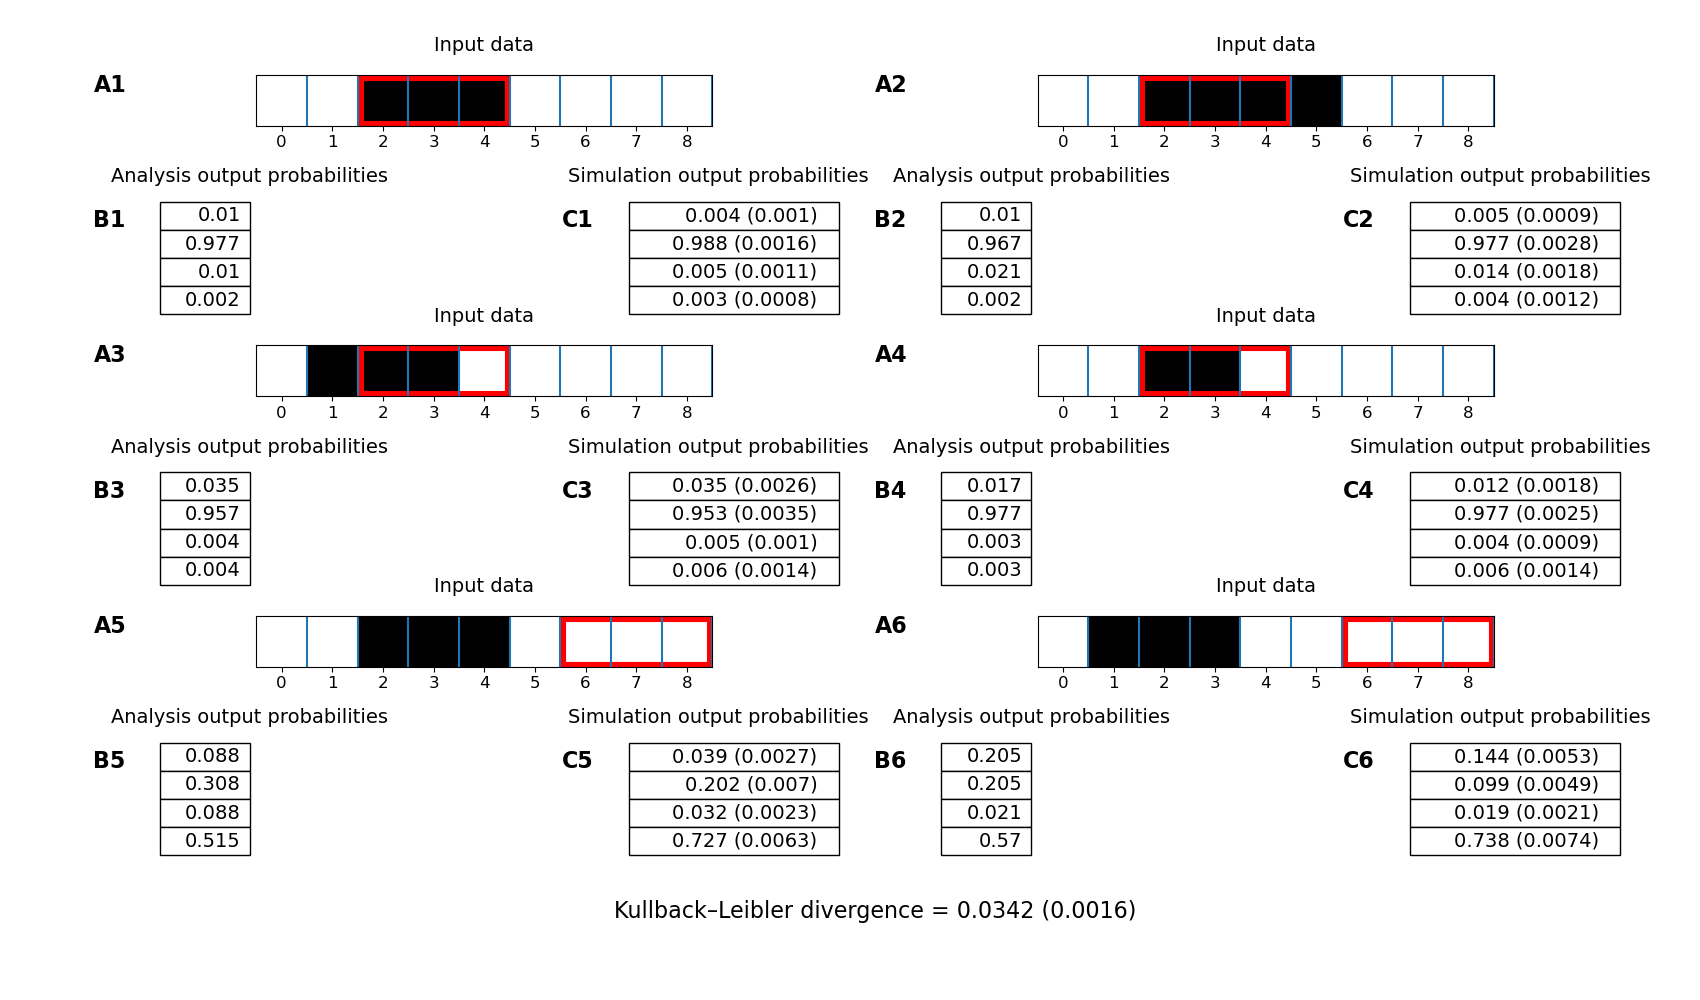
\includegraphics[width=\linewidth]{figures/1D/training/trainingEvaluation_98_440_4_c3.png}
  \caption{\textbf{Analysis and simulation result. Parameters: } $f_{input} = 98 Hz, f_{prior} = 440 Hz, \tau_{decay} = 4 ms, c = 3$ \textbf{A} Input images with 9 x 1 pixels. \textbf{B} Analytically calculated posterior probabilities. \textbf{C} Proportions of the spikes of the output neurons during the simulation and their standard deviations in brackets.}
  \label{fig:1DTrainingEvaluationC3}
\end{figure}

\subsection{Discussion}

Using the previously determined optimal network parameters for the weight training process was successful. When comparing A with B and C with D in Figure \ref{fig:1DTraining} it can be seen that the network learned the correct discrimination function. However the size the weights and the prior weights is too small. The Kullback-Leibler divergence also was worse with 0.0625 compared to 0.0101 from Experiment 5 Figure \ref{fig:1D_98_440_4}.
To try to improve the similarity of the learned and the calculated probability matrices, and also to minimize the Kullback-Leibler divergence, different values for the weight shifting parameter c were tried. The lowest Kullback-Leibler divergence was achieved with $c = 3$. For this c the divergence was 0.0342. When comparing  the probability matrices in Figure \ref{fig:1DTrainingC3} it is apparent that the values of the learned $P^{X|Y}$ are still to small and they could profit from further increasing c. On the other hand the values in the learned $P^{Y|Z}$ are already too big and would profit from a smaller c. If one would want to further minimize the Kullback-Leibler divergence two separate weights shifting parameters for the input weights and the prior weights could be implemented.